\documentclass[12pt]{book}
\pagestyle{empty}
\usepackage{amsmath, amssymb, amsthm}
\usepackage{latexsym, epsfig, ulem, cancel, multicol, hyperref}
\usepackage{graphicx, tikz, subfigure,pgfplots}
\usepackage[margin=1in]{geometry}
\setlength{\parindent}{0pt}
\usepackage{multirow}
\usepackage{mathtools}


\usepackage{verbatim}
\usepackage{tikz}
\usepackage{pgfplots}

\newcommand{\wsnumber}{1}
\newcommand{\wstopic}{Vectors}
\pgfplotsset{
    every linear axis/.append style={
       axis x line=center,
       axis y line=center,
       xlabel={$x$},
       ylabel={$y$}
    },
    every axis plot/.append style={thick,mark=none}
}
\tikzset{
    point/.style={circle,draw,fill,minimum width=0.3ex,inner sep=0pt,outer sep=0pt},
    every label/.append style={black}
}


\usepackage[margin=1in]{geometry}
\usepackage{amsmath, amssymb, amsthm, graphicx, hyperref}
\usepackage{enumerate}
\usepackage{fancyhdr}
\usepackage{multirow, multicol}
\usepackage{tikz}
\pagestyle{fancy}
\fancyhead[RO]{Dennis Li}
\fancyhead[LO]{$\bigoplus$}
\usepackage{comment}
\newif\ifshow
\showfalse

\ifshow
  \newenvironment{solution}{\textbf{Solution.}}{}
\else
  \excludecomment{solution}
\fi

\renewcommand{\thefootnote}{\fnsymbol{footnote}}
\usepackage{comment}

\newcommand{\T}[0]{\top}
\newcommand{\F}[0]{\bot}
\newcommand{\liminfty}[1]{\lim_{#1 \to \infty}}
\newcommand{\limzero}[1]{\lim_{#1 \to 0}}
\newcommand{\Z}{\mathbb{Z}}
\newcommand{\R}{\mathbb{R}}
\newcommand{\C}{\mathbb{C}}
\newcommand{\Q}{\mathbb{Q}}
\newcommand{\odd}[0]{\mathbb{Z} - 2\mathbb{Z}}
\newcommand{\lineint}[1]{\int_{#1}}
\newcommand{\pypx}[2]{\frac{\partial #1}{\partial #2}}
\newcommand{\divg}{\nabla \cdot}
\newcommand{\curl}{\nabla \times}
\newcommand{\dydx}[2]{\frac{d #1}{d #2}}
\newcommand{\sqbkt}[1]{\left[ #1 \right]}
\newcommand{\paren}[1]{\left( #1 \right)}
\newcommand{\tribkt}[1]{\left< #1 \right>}
\newcommand{\abso}[1]{\left|#1 \right|}
\newcommand{\zero}{\{0\}}
\newcommand{\then}{\rightarrow}
\newcommand{\nonneg}{\Z^+ \cup \{0\}}
\DeclarePairedDelimiter\ceil{\lceil}{\rceil}
\DeclarePairedDelimiter\floor{\lfloor}{\rfloor}
\newcommand{\union}[2]{\bigcup_{#1}^{#2}}
\newcommand{\inter}[2]{\bigcap_{#1}^{#2}}
\newcommand{\openclose}[1]{\left( #1 \right]}
\newcommand{\closeopen}[1]{\left[ #1 \right)}

\newcommand{\defcomp}{\exists r,s\in \Z^+ \paren{n=rs \wedge \paren{1<r<n} \wedge \paren{1<s<n}}}
\newcommand{\defprime}{\forall r,s \in \Z ^+ \paren{n=rs \rightarrow \paren{r = 1 \wedge s = n}\veebar \paren{r=n \wedge s=1}}}


\newtheorem*{remark}{Remark}


\begin{document}

\begin{center}
\ifshow
  \textbf{\Large Homework 0 Solution}\\
\else
  \textbf{\Large Discrete Math Notebook}\\
\fi
Dennis Li\\Instructor: Ken Cereste\\
\end{center}

\hrule

\vspace{0.2cm}

\begin{enumerate}[$\bullet$]  
\item A Notebook for MA-UY 2314 Discrete Math during Summer 6W2 2024. 
\end{enumerate}

\hrule

\vspace{0.5cm}

\tableofcontents


\chapter{Discrete Math - Epp}
\section{Statements and Operators}
A statement is something that is true or false. A statement variable, or a prepositions is a variable that represents the statement. 
\subsection{Tautology and Contradiction}
\begin{enumerate}
    \item[$\top$] A tautology is something that is always true, sometimes denoted as \textbf{t}
    \item[$\bot$] A contradiction is something that is always false, sometimes denoted as \textbf{c}
\end{enumerate}
\subsection{Logical Operators}
\begin{enumerate}
    \item[$\neg$] A negation is something that flips the truth value of a statement variable
    \[
    \begin{tabular}{|c|c|}
        \hline
        $p$ & $\neg p$\\
        \hline
        T&F\\
        \hline
        F&T\\
        \hline
    \end{tabular}
    \]

    \item[$\vee$] Disjunction, basically \textit{or}
    \[
    \begin{tabular}{|c|c|c|}
        \hline
        $p$ & $q$ & $p \vee q$\\
        \hline
        T&T&T\\
        \hline
        T&F&T\\
        \hline
        F&T&T\\
        \hline
        F&F&F\\
        \hline
    \end{tabular}
    \]
    
    \item[$\wedge$] Conjunction, basically \textit{and}
    \[
    \begin{tabular}{|c|c|c|}
        \hline
        $p$ & $q$ & $p \wedge q$\\
        \hline
        T&T&T\\
        \hline
        T&F&F\\
        \hline
        F&T&F\\
        \hline
        F&F&F\\
        \hline
    \end{tabular}
    \]
    
    \item[$\rightarrow$] Conditional, \textit{if $\ldots$ then}\\
    \[
    \begin{tabular}{|c|c|c|}
        \hline
        $p$ & $q$ & $p \rightarrow q$\\
        \hline
        T&T&T\\
        \hline
        T&F&F\\
        \hline
        F&T&T\\
        \hline
        F&F&T\\
        \hline
    \end{tabular}
    \]
    \[
    \neg ( p \rightarrow q ) =  p \wedge \neg q
    \]

    \item[$\leftrightarrow$] Bi-conditional, basically \textit{if and only if}
    \[
    \begin{tabular}{|c|c|c|}
        \hline
        $p$ & $q$ & $p \leftrightarrow q$\\
        \hline
        T&T&T\\
        \hline
        T&F&F\\
        \hline
        F&T&F\\
        \hline
        F&F&T\\
        \hline
    \end{tabular}
    \]
    \[
    \neg (p \leftrightarrow q) \equiv p \leftrightarrow \neg q \equiv p \oplus q
    \]
    

    \item[Op. Order] $\neg \xrightarrow{then} \vee \; \& \; \wedge \xrightarrow{then}\;\; \rightarrow \& \leftrightarrow$

    \item[Truth Table] $p\vee (q \wedge r) \equiv (p\vee q)\wedge(p \vee r)$
        \[
            \begin{tabular}{|c|c|c|c|c|c|c|c|}
            \hline
            $p$ & $q$ & $r$ & $q \wedge r$ & $p \vee (q \wedge r)$ & $p \vee q$ & $p \vee r$ & $(p \vee q) \wedge (p \vee r)$\\
            \hline
            T&T&T&T&\textbf{T}&T&T&\textbf{T}\\
            \hline
            T&T&F&F&\textbf{T}&T&T&\textbf{T}\\
            \hline
            T&F&T&F&\textbf{T}&T&T&\textbf{T}\\
            \hline
            T&F&F&F&\textbf{T}&T&T&\textbf{T}\\
            \hline
            F&T&T&T&\textbf{T}&T&T&\textbf{T}\\
            \hline
            F&T&F&F&\textbf{F}&T&F&\textbf{F}\\
            \hline
            F&F&T&F&\textbf{F}&F&T&\textbf{F}\\
            \hline
            F&F&F&F&\textbf{F}&F&F&\textbf{F}\\
            \hline
            \end{tabular}
        \]
    
\end{enumerate}


\newpage
\subsection{Proofs}
How to write Proofs, here is a sample\\
Show that $[(p \rightarrow q) \wedge (p \rightarrow \neg q)] \rightarrow \neg p$ is a tautology.
\begin{proof}
    \begin{align*}
        \text{let } & \text{$p$, $q$, and $r$ be statement variables and $r \equiv \neg p$}\\
        & [(p \rightarrow q) \wedge (p \rightarrow \neg q)] \rightarrow \neg p & \text{Substitution} \\
        \equiv &  [(p \rightarrow q) \wedge (p \rightarrow \neg q)] \rightarrow r \\
        \equiv & [(\neg p \vee q) \wedge (\neg p \vee \neg q)] \rightarrow r & \text{Theorem *}\\
        \equiv & [(r \vee q) \wedge (r \vee \neg q)] \rightarrow r & \text{Substitution} \\
        \equiv & [ r \wedge (q \vee \neg q )] \rightarrow r & \text{Distributivity}\\
        \equiv & [r \wedge \T ] \rightarrow r & \text{Negation Law}\\
        \equiv & r \rightarrow r & \text{Identity Law}\\
        \equiv & \neg r \vee r & \text{Theorem *}\\
        \equiv &  r \vee \neg r & \text{Commutativity}\\
        \equiv & \T & \text{Negation Law}
    \end{align*}
    \[
    \therefore [(p \rightarrow q) \wedge (p \rightarrow \neg q)] \rightarrow \neg p \equiv \T
    \]
\end{proof}

\subsection{Inverses}
Let $p$ and $q$ be statement variables. 
    \[
    p \rightarrow q
    \]
\begin{enumerate}
    \item[Contrapositive] 
    \[
    \neg q \rightarrow \neg p
    \]
    \item[Converse]
    \[
    q \rightarrow p
    \]
    \item[Inverse]
    \[
    \neg p \rightarrow \neg q
    \]
    Notice that the inverse is the contrapositive of the Converse.
    \item[Properties] A statement is logically equivalent to its contrapositive.

\end{enumerate}

\subsection{Inequalities}
Different cases of inequalities
\begin{enumerate}
    \item[<, >] strict
    \item[$\leq,\; \geq$] weak
    \item[a<b<c] chained. Be careful of its negation
    \[
    a<b<c \xrightarrow{negate} b\geq c \vee b\leq a
    \]
\end{enumerate}

\subsection{Arguments}
An argument is a sequence of statements, and an argument form is a sequence of statement forms. All statements in an argument and all statement forms in an argument form except for the final one, are called premises, assumptions, or hypotheses. The final statement of statement form is called the conclusion. It basically looks like as follows:
\begin{align*}
    \because & e > 1\\
    & e < 3\\
    \therefore & 1<e<3
\end{align*}
Stuff after $\therefore$ symbol is the conclusion. 

\subsubsection{Critical Roll}
Check the truth table to find a row where all statement variables are true, and observe the result.
\subsubsection{Generalization}
\subsubsection{Fallacies}
A fallacy is an error in reasoning that results in an invalid argument these common fallacies are using ambiguous premises, circular arguments, and etc. If your arguments are bad and contains error, we called it a fallacy.
\subsubsection{Errors}
\subsubsection{Validity vs. Truth}
Validity is a property of an argument.\\
Truth is a property of a statement.
\subsubsection{sound}
An argument is called sound if and only if it is valid and all its premises are true. An argument that is not sound is called unsound. 
\subsubsection{Proof by Contradiction}
If we can show that the assumption $p$ is false leads logically to a contradiction, then we can conclude that $p$ is true. 
\[
\neg p \rightarrow \F
\]
\[
\therefore p
\]\\
\begin{enumerate}
    \item 
\end{enumerate}

\subsubsection{Premise \& Conclusion}


\subsection{Useful Formulas}
    \begin{enumerate}
        \item $\neg (p \rightarrow q) \equiv p \wedge \neg q$
    \end{enumerate}




\section{Predicate and Qualifiers}
\subsection{Symbols}
    \subsubsection{Sets}
        \begin{enumerate}
            \item[$\varnothing$] empty set
            \item[$\mathbb{Z}$] set of all integers
            \item[$\mathbb{Z}^+$] set of all positive integers
            \item[$2\mathbb{Z}$] set of all even integers
            \item[$\mathbb{Z} - 2\mathbb{Z}$] set of all odd integers
            \item[$\mathbb{R}$] set of all real numbers
            \item[$\mathbb{C}$] set of all complex numbers
            \item[$\mathbb{H}$] set of all quaternions
            \item[$\mathbb{Q}$] set of all rational numbers
        \end{enumerate}
    \subsubsection{operators}
    Let $A$,$B$ be sets
        \begin{enumerate}
            \item[$A\in B$] A in B
            \item[$A\notin B$] A not in B
            \item[$\{a_1,a_2\ldots\}$] set with elements $a_1,a_2\ldots$
            \item[$A^c$] A compliment
            \item[$A \subseteq B$] A is a subset of B
            \item[$A \not\subseteq B$] A is not a subset of B
                \[
                1
                \]
            \item[$A \cup B$] A union B
                \[
                \{x\in U: x\in A \text{ or } x \in B\}
                \]
            \item[$A \cap B$] A intersect B
                \[
                \{x\in U: x\in A \text{ and } x \in B\}
                \]
            \item[$A - B$] set difference of A minus B\\
                \[
                A - B: \{ x \in U: x\in A \text{ and } x \notin B\}
                \]
                \[
                A - B \coloneqq \{x\in A: x\notin B\}
                \]
            \item[$N(A)$ \& $|A|$] Cardinality of A
            \item[$P(A)$] power set of A
        \end{enumerate}
        
\subsection{Predicates and Quantifiers I}
\subsubsection{Predicate}
    A \textbf{Predicate} is a sentence that contains a finite number of variables and becomes a statement when specific values are substituted for the variables. The \textbf{domain} for a predicate variable is the set of all values that may be substituted in place of the variable. 
    \[
    \{ x\in D: P(x) \} = \{ x\in D: P(x) \equiv \T \}
    \]
\subsubsection{What are Predicates}
    Here are some examples\\
    \begin{enumerate}
        \item let $P_1(x)$ be the predicate \textit{x is even with the domain $\mathbb{Z}^+$}\\
        Replace the $x$ with integers to see if the the generated statement is true.
        \[
        \{ n\in \mathbb{Z} : \exists k \in \mathbb{Z}^+ (n=2k) \}
        \]
        This set allows $P_1(x)$ to always be true\\
        \item let $P_2(x)$ be the predicate $x \leq \frac{1}{x}$ with the domain ${x\in \mathbb{R}: 0 < x < \infty}$. Find the set that makes $P_2(x)$ always true.\\
        \item let $P_3(x)$ be the predicate $\sin x \geq 0$
    \end{enumerate}
    
\subsubsection{Qualifiers}

\begin{enumerate}
    \item[$\forall$] is called the \textbf{universal qualifier}
    \item[$\exists$] is called the \textbf{existential qualifier}
    \item[$\exists !$] there exist a unique
\end{enumerate}

\subsection{Statements with qualifiers}
\begin{enumerate}[a.]
    \item $\forall x \in \mathbb{Z}\left( \sqrt{x^2}=x \right)$
        \item[disproof.] $ \sqrt{\paren{-1}^2} = 1 \neq -1$\\
        \qed
    \item $\forall x \in \Z^+ \paren{\sqrt{x^2}=x}$
    \item $\exists x \in \R - \{0\}\paren{x = \frac{1}{x}}$
        \item[proof.] Choose $1 \in \R - \{ 0 \} \paren{1=\frac{1}{1}}$\\
        \qed
    \item $\exists x \in \Q \paren{x^2 = 2} $
        \item[disproof.]$x^2 = 2$\\
                    $x = \pm \sqrt{2}$\\
                    $\sqrt{2} \notin \Q$\\
                    \qed
    \item $\exists x \in \Q \; \forall y \in \Q \paren{xy=yx=y}$
        \item[proof.] Choose $1 \in \Q$, let $y \in \Q$ \ldots
    \item $\forall x \in \Q - \{0\} \; \exists y \in \Q \paren{xy=yx=1}$
            \\ \qed
        \item[proof.] let $x \in \Q -\{0\}$, $\exists m,n \in \Z -\{0 \}\paren{x = \frac{m}{n}}$ by definition of rational numbers\\
        \(
        \text{choose } y \coloneqq \frac{1}{x} = \frac{n}{m}
        \)
        \[
        xy = x\paren{\frac{1}{x}} = \paren{\frac{m}{n}} \paren{\frac{n}{m}}
        =1 = \paren{\frac{n}{m}}\paren{\frac{m}{n}} = \paren{\frac{1}{x}}x = yx
        \]
        \qed
    \item $\exists x \in \Z \; \forall y \in \Z \paren{xy=yx=1}$
        \item[disproof.]we first negate the statement 
        \[
        \neg \; \exists x \in \Z \; \forall y \in \Z \paren{xy=yx=1}
        \]
        \[
        \equiv \forall x \in Z \; \exists y \in Z \paren{xy=yx \vee yx=1}
        \]
        let $x \in Z$, choose $0 \in \Z$.\\
        \[
        0x=0\neq 1
        \]
        \qed
\end{enumerate}
\subsection{Statements with Words}
\begin{enumerate}[a.]
    \item For any complex number $z$, the modulus (or absolute value) of $z$ is non-negative
    \[
    \forall z \in \C \paren{\abso{z} \geq 0}
    \]

    \item There exists a complex number $z$ such that $z^2 < 1$
    \[
    \exists z \in \C \paren{z^2 <-1}
    \]
\end{enumerate}

\subsection{Universal Conditional Statements}
A universal conditional statement takes form
\[
\forall x \paren{P(x) \rightarrow Q(x)}
\]

\begin{enumerate}[a.]
    \item $forall x \in \R \paren{\abso{x}=0 \rightarrow x=0}$
    
    \item $\forall z \in \C \paren{z = \Bar{z} \rightarrow z \notin \R}$
    
    \item[Theorem] 
    $\forall z \in \C - \{0\}\paren{z = \Bar{z} \rightarrow z \notin \R}$
        \begin{proof}[Proof 2-1]
        $\forall z \in \C - \{0\}\paren{z = \Bar{z} \rightarrow z \notin \R}$\\
            let $z \in \C - \{0 \}$, and let $z = a+bi \; \{ a,b \in \R :a \neq 0 \vee b \neq 0 \}$\\
            suppose $z = - \Bar{z}$, then\\
            \begin{align*}
                &a+bi = -a+bi\\
                &a+a =0\\
                &a = 0
            \end{align*}
            recall \(
            \{ a,b \in \R :a \neq 0 \vee b \neq 0 \}
            \), and since $a=0$, therefore $b\neq 0$ by contradiction.\\
            \[
            \therefore z = a+bi = bi \notin \R
            \]
        \end{proof}
        \newpage
\end{enumerate}

\subsection{Equivalent Form of Statements}
If $P(x)$ and $Q(x)$ are predicates, and B is a set such that $A\coloneqq \{ x\in B : P(x) \equiv \T \}$, then $A \subseteq B$, and we can rewrite
\[
\forall x \in B \paren{P(x) \rightarrow Q(x)}
\]
as
\[
\forall x \in A \paren{Q(x)}
\]
\begin{enumerate}[a.]
    \item All integers are rational numbers
        \begin{align*}
                    &\forall x \in \R \paren{x \in \Z \rightarrow x \in \Q}\\
            \equiv  & \forall x \in \Z \paren{x \in \Q}
        \end{align*}
        if $x$ is an integer, it is a rational number.
    
\end{enumerate}
\subsection{Special Notation}
\begin{enumerate}
    \item[$\Rightarrow$] means $\forall x \paren{ P(x) \rightarrow Q(x)}$
    \item[$\iff$] means $\forall x \paren{ P(x) \iff Q(x)}$
\end{enumerate}

\subsection{Predicates \& Quantifiers II}
\begin{enumerate}
    \item $\neg \forall x(P(x)) \equiv \exists x (\neg P(x))$ 
\end{enumerate}
\subsubsection{Examples}
    \begin{enumerate}[a.]
        \item $\forall x \in \R (\sin x < -1)$\\
        \item[$\neg$] $\forall x \in \R (\sin x < -1)$
             \begin{align*}
                 \neg    & \forall x \in \R (\sin x < -1)\\
                 \equiv  & \exists x \in \R (\sin x \geq -1)
             \end{align*}
         \item All real numbers are transcendental 
         \item[$\neg :$] There exists real numbers that are not transcendental.
         \item[or] There exists real numbers that are algebraic
    \end{enumerate}
\newpage
\subsubsection{Relationships}
let $A = \{x_1, x_2, \ldots x_n \}$
\[
\forall x \in A (P(x)) \equiv P(x_1) \wedge P(x_2)\wedge \ldots P(x_n)
\]
\[
\exists x \in A (P(x)) \equiv P(x_1) \vee P(x_2) \vee \ldots P(x_n)
\]
Negation of qualifiers flip them, with out changing the $\in$ to $\notin$
\[
\neg \forall x \Rightarrow \exists x
\]
\subsubsection{Transcendental}
\begin{enumerate}
    \item For any real number c, there exists a polynomial p with rational coefficients, such that c is \textbf{algebraic} if and only if $p(c)=0$
    \[
    \forall c \in \R \; \exists p \in \Q [x] \paren{c \textbf{ is algebraic } \leftrightarrow p(c) = 0)}
    \]
    its negation is
    \[
    \exists c \in \R \; \forall p \in \Q [x] \paren{c \textbf{ is algebraic } \leftrightarrow p(c) \neq 0)}
    \]
    \item For any real number c, such that, for any polynomial $p$ with rational coefficients, c is \textbf{transcendental} if and only if $p(c)=0$
    \[
    \exists c \in \R \; \forall p \in \Q [x] \paren{c \textbf{ is transcendental } \leftrightarrow p(c) \neq 0)}
    \]
\end{enumerate}

\subsection{Statement with Qualifiers}
A \textbf{Universal Instantiation} is true of everything in a set, then it is true of any \textbf{particular} element in the set.\\
\\
A \textbf{Universal Modus Ponens}
\[
\forall x \paren{P(x) \rightarrow Q(x)}
\]
\[
\textbf{then } \forall x \in P(x) \paren{Q(x)} 
\]
To say an \textit{argument form} is valid means: No matter what particular predicates are substituted for the predicate symbols in its premises, if the resulting premise statements are all true, then the conclusion is also true. An argument is called \textbf{valid} if and only if its form is valid. It is called \textbf{sound} if and only if its form is valid and its premises are true. 

A \textbf{Converse Error} is as follows
\[
\forall x \paren{p(x) \rightarrow Q(x)} \\
Q(a)\\
\therefore P(x)
\]
Example being, all rational numbers are algebraic, c is algebraic. The counter example is $\sqrt{2}$, which is algebraic but irrational. However, the converse is true. All rational numbers are algebraic. \\

An \textbf{Inverse Error} is when you inverse something, the statement is erroneous. Just like above. \\

A \textbf{Universal Transitivity} is described as follows:
\[
\forall x \paren{ P(x) \rightarrow Q(x)}
\]
\[
\forall x \paren{ Q(x) \rightarrow R(x)}
\]
Then
\[
\forall x \paren{ P(x) \rightarrow R(x)}
\]

\subsubsection{Theorem Algebraic}
All rational numbers are algebraic.
\[
\forall q \in \Q \paren{\text{q is algebraic}}
\]
rewrites
\[
\forall q \in \Q \; \exists p \in \Q [x] \paren{p(q)=0}
\]
\begin{proof}[Pf. Q]
    let $q \in \Q$, There exist $m \in \Z$ and $n \in \Z - \{0\} $ such that $p = \frac{m}{n}$. Choose $p(x) = nx - m \in \Q [x]$ such that 
    \[
    p(x) = p\paren{\frac{m}{n}} = \\
    n\paren{\frac{m}{n}}-m = 0
    \]
\end{proof}

\subsubsection{Theorem Algebraic 2}
\[
\forall x \in \Q \paren{x \text{ x is algebraic}}
\]
\[
\equiv \forall x \in R \paren{x \in Q \rightarrow x \text{ is algebraic}}
\]
We can write its converse
\[
\forall x \in R \paren{\text{x is transcendental } \rightarrow x \notin Q}
\]
This is called a \textbf{Corollary}, or the consequence of another theory:\\
\[
\textit{All transcendental numbers are irrational}
\]

\newpage
\section{Methods of Proofs}
\subsection{Things we accept}
\begin{enumerate}
    \item We assume a familiarity with the laws of basic algebra listed in Appendix A of the textbook.
    \item  The Equivalence Relation 
        \begin{enumerate}[i.]
            \item Reflexivity: $A=A$
            \item Symmetry: $A=B \leftrightarrow B=A$
            \item Transitivity: $A=B \wedge B=C \rightarrow A=C$
        \end{enumerate}
    \item We use the principle of substitution:\\
            For all objects $A$ and $B$, if $A=B$, then we may substitute B wherever we have $A$.
    \item Defining Characteristics\\
    We assume the there is no integer between 0 and 1. And we assume the set of integers are closed under \textit{addition}, \textit{subtraction}, and \textit{multiplication.}
        \begin{enumerate}[i.]
            \item $\neg \exists x \in \Z \paren{0<x<1}$
            \item $\forall x,y \in Z \paren{x+y  \in \Z}$
            \item $\forall x,y \in \Z \paren{x-y \in \Z}$
            \item $\forall x,y \in Z \paren{xy   \in \Z}$
        \end{enumerate}
\end{enumerate}

\subsection{Numbers}
\begin{enumerate}
    \item even number
        \[
        \{ n \in \Z : \forall k \in \Z \paren{n = 2k} \}
        \]
    \item odd number
        \[
        \{ n \in \Z : \forall k \in \Z \paren{n = 2k+1} \}
        \]
    \item prime number
        \[
        \forall r,s \in \Z ^+ \paren{n=rs \rightarrow \paren{r = 1 \wedge s = n}\veebar \paren{r=n \wedge s=1}}\}
        \]
    \item composite number
        \[
        \exists r,s \in \Z ^+ \paren{n=rs \wedge \paren{1<r<n} \wedge \paren{1<s<n}} \}
        \]
\end{enumerate}

\subsubsection{Sample Proof}
\begin{enumerate}[a.]
    \item $\forall r,s \in \Z \paren{6r+4s^2 +3 \in \Z - 2\Z}$
        \begin{proof} let $r,s \in \Z$.
            \begin{align*}
            6r+4s^2 +3  & = 6r +4s^2 +2 +1 \\
                        & = 2 (3r + 2s^2 +1) +1 
            \end{align*}
        Define $k\coloneqq 3r+2s^2 +1 \in Z$ since $\Z$ is closed under products and sums, so that 
        \[
        2 (3r + 2s^2 +1) +1 = 2k+1 \in \Z - 2\Z
        \]
        \end{proof}
    \item $\forall r,s \in Z \paren{r^2 + 2rs + s^2 \in \Z ^+ - \mathbb{P}}$
        \begin{proof} Composite number is defined by the set
        \[
        \exists x,y \in \Z ^+ \paren{n=xy \wedge \paren{1<x<n} \wedge \paren{1<y<n}}
        \]
        let $r,s \in \Z ^+$\\
            \begin{align*}
                r^2 + 2rs + s^2 
                &= (r+s)^2\\
                &=(r+s)(r+s)
            \end{align*}
            \[
            \because r,s\in \Z ^+ 
            \]
            \[
            1 \leq r \leq r^2
            \]
            \[
            1 \leq s \leq s^2
            \]
            \[
            1< 2 \leq r+s \leq r^2 + s^2 < r^2 + 2rs + s^2
            \]
            
        \end{proof}
    \item Theorem 4.1.1\\
        The sum of any two even numbers is even.
        \[
        \forall m,n \in 2\Z \paren{m+n \in 2\Z}
        \]
        \begin{proof}let $m,n \in 2\Z$
            \begin{align*}
                &m = 2k_1 \textit{ for some }\; k_1 \in \Z\\
                &m = 2k_2 \textit{ for some }\; k_2 \in \Z\\
                &m+n = 2\paren{k_1 + k_2}\\
                &k_3 \coloneqq k_1 + k_2 \in \Z 
                &\text{Integers closed under addition}\\
                \therefore & m+n = 2k_3 \in 2\Z
            \end{align*}
        \end{proof}
\end{enumerate}

\subsection{Methods of Direct Proof}
\begin{enumerate}
    \item express the statement as a universal conditional 
        \[
        \forall x \in A (P(x) \rightarrow Q(x))
        \]
    \item suppose $a \in A$ is a particular but arbitrarily chosen element such that $P(a)$ is true.
        \[
        \textit{let } a\in A \textit{. Suppose }P(a).
        \]
    \item Show $Q(a)$ is true using definitions, theorems, or rules for logical inference. 
    \item since $a \in A$ was arbitrarily chosen, generalize to $x$ so that 
        \[
        \forall x \in A (P(x) \rightarrow Q(x))
        \]
\end{enumerate}
\subsection{Directions of Proof}
\begin{enumerate}
    \item Copy the statement of the theorem
    \item Clearly mark the beginning of your proof
    \item make your proof self-contained
    \item write your proof in complete, grammatically correct sentences
    \item keep your reader informed about the status of each statement in your proof
    \item give a reason for each assertion in your proof
    \item include words and phrases that make the logic of your arguments clear
    \item display equations and inequalities
\end{enumerate}


\subsubsection{example 4.2.1}
    The difference of any odd integer and any even integer is odd
    \[
    \forall m \in \Z - 2\Z \; \forall n \in 2\Z \paren{m-n \in \Z - 2\Z}
    \]
    \begin{proof}
        let $m$ be odd and is defined by
        \[
        m=2k_1 + 1 \; \textit{ for some } k_1 \in \Z - 2\Z
        \]
        let $n$ be even and is defined by 
        \[
        n=2k_2 \; \textit{ for some } k_2 \in \Z
        \]
        The difference can be expressed as
        \begin{align*}
            m-n &= 2k_1+1-2k_2 & \text{Substitution} \\
                &=2(k_1-k_2)+1 & \text{by algebra}
        \end{align*}
        let $k_1-k_2 = k_3 \in \Z$ since integers are closed under subtraction, then
        \[
        m-n = 2k_3+1 \in \Z - 2\Z
        \]
    \end{proof}

\subsubsection{example 4.2.3}
There is a positive integer n such that $n^2+3n+2$ is prime.\\
The definition of composite number $n$ is
\[
\defcomp
\]
\begin{proof}
    let $n \in \Z^+$\\
    \[
    n^2+3n+2=(n+1)(n+2)
    \]
    Since $n\in \Z^+$, $0<1\leq n \leq n^2$
    \[
    1<2\leq n+1 < n+2 < 3n+2 < n^2 +3n +2
    \]
    Therefore $n^2 +3n +2$ is a composite number and not a prime.
\end{proof}

\subsubsection{example 4.2.10}
If $n$ is any even integer, then $(-1)^n=1$
\begin{proof}[proof E]
    let $ n \in 2\Z$\\
    $n=2k$ for some $k \in \Z$\\
    \[
    (-1)^n = (-1)^{2k} = \paren{\paren{-1}^2}^k = 1^k = 1
    \]
\end{proof}
If $n$ is any odd integer, then $(-1)^n=-1$
\begin{proof}[proof F]
    let $n \in \Z - 2\Z$\\
    $n = 2k+1$ for some $k \in \Z$
    \begin{align*}
    &(-1)^n = (-1)^{2k+1} \\
    =& (-1)(-1)^{2k} & \text{By Algebra}\\
    =& (-1) \times 1 &\text{By Proof E}\\
    =&-1
    \end{align*}
    
\end{proof}

\subsection{Rational and Irrational}
\subsubsection{Rational Number}
\[
q\in \Q \iff \exists m\in \Z \; \exists n \in \Z - \{0\}
\paren{q = \frac{m}{n}}
\]
\subsubsection{Irrational Number}
\[
q \in \mathbb{I} \iff \forall m \in \Z \; \forall n \in \Z - \{0\}
\paren{q\neq \frac{m}{n}}
\]
\subsubsection{Zero Product Property}
Let $X$ be either $\Z, \Q, \R, \C$, If $x_1 \ in X$ and $x_2 \in X$ are non-zero, then their product $x_1x_2$ is non-zero. 
\[
\forall x_1, x_2 \in X 
\paren{x_1 \neq 0 \wedge x_2 \neq 0 \rightarrow x_1x_2 \neq 0}
\]

\subsubsection{Theorem 4.3.2}
\[
\forall p,q \in \Q \paren{p+q \in \Q}
\]
\begin{proof}[proof 4.3.2]
\begin{align*}
    &\text{let $p,q \in Q$}\\
    &p \in \frac{m_1}{n_1}\\
    &q \in \frac{m_2}{n_2}\\
    &\text{for some $m_1,m_2 \in \Z$ and some } \text{$n_1,n_2\in \Z - \{0\}$}&\\
    p + q &= \frac{m_1}{n_1} + \frac{m_2}{n_2}\\
    p+q & = \frac{m_1n_2 + m_2n_1}{n_1n_2}
\end{align*}
    $m_1n_2 + m_2n_1 \in \Z$ since $\Z$ is closed under products and sums.\\
    $n_1n_2 \in \Z - \{0\}$ since $\Z$ is closed under products and non-zero via Zero Product Property\\
    \[
    \therefore p+q \in \Q
    \]
\end{proof}
\subsection{Corollary 4.3.2}
The argument is proofed
\[
\forall q \in \Q \paren{2q \in \Q} \equiv
\forall q \in \Q \paren{q+q \in \Q}
\]


\newpage
\subsubsection{Practise 19}
Proof that
\[
\forall a,b\in \R \paren{a<b \rightarrow a< \frac{a+b}{2}<b}
\]
Try negate it
\[
\exists a,b\in \R \paren{a<b \wedge 
\paren{a\geq \frac{a+b}{2} \vee b \geq \frac{a+b}{2}}}
\]
\begin{proof}[proof 4.3.19]:\\

    let $a,b \in \R$. Suppose $a<b$. \\
    \begin{align*}
        a& <b\\
        a + a &< a +b\\
         2a &< a+b\\
         a &< \frac{a+b}{2}\\
         a+b &< b+b\\
         a+b &< 2b\\
         \frac{a+b}{2} &< b\\
        \therefore  a & <\frac{a+b}{2}<b & \text{Conjunction}
    \end{align*}
    
\end{proof}

\subsubsection{Practise 28}
    Suppose $a,b,c,d \in \Z$ and $a \neq c$. Suppose also that $x \in \R$ satisfying the equation
    \[
    \frac{ax+b}{cx+d}=1
    \]
    Must $x$ be rational? if so, express x as a ratio of integers. 
    \[
    \forall a,b,c,d  \in \Z \; \forall x \in \R 
    \paren{a\neq c \wedge \frac{ax+b}{cx+d}=1 \rightarrow x \in \Q}
    \]
    \begin{proof}[proof 4.3.28]:\\
    
    let $a,b,c,d \in \Z$ and $x \in \R$
    \begin{align*}
        \frac{ax+b}{cx+d}&=1\\
        ax+b &= bx+c\\
        x(a-c)&= d-b\\
        x &= \frac{d-b}{a-c} & a\neq c 
    \end{align*}
        $d-b, a-c \in \Z$ since $\Z$ is closed under subtraction and $a-c \neq 0$.
        \[
        \therefore x \in \Q
        \]
    \end{proof}

\subsection{Direct Proof by Contradiction III}
\subsubsection{Divisible}
$d\mid n$ means $d$ divides $n$, or $d$ is divisible by $n$, and vice versa.
\[
d \mid n \iff \exists k \in \Z \paren{n=dk \wedge d\neq 0}
\]
\[
d \nmid n \iff \forall k \in \Z \paren{ n\neq dk \vee d = 0}
\]
\subsubsection{Divisions of Zero}
Anything divides zero, nothing is divisible by zero. 
\[
\forall k \in \Z - \{0\} \paren{k \mid 0}
\]

\subsubsection{Theorem 4.1.1}
\[
\forall m,n\in \Z 
\paren{m>0 \wedge n>0 \wedge m \mid n \rightarrow m \leq n}
\]
is logically equivalent to
\[
\forall m,n \in \Z^+ \paren{
m \mid n \rightarrow m \leq n}
\]


\subsubsection{Property T25}
\[
\forall a,b  \in \R 
\paren{ab>0 \rightarrow\paren{a>0 \wedge b>0} \vee \paren{a<0 \wedge b<0}}
\]

\newpage

\subsubsection{Theorem 4.4.2}
The \textbf{\textit{only}} divisors of 1 are 1 and $-1$.
\begin{proof}[proof 4.4.2]:\\
    \begin{align*}
        1 \mid 1\\
        -1 \mid 1\\
    \end{align*}
    Proof that 1 and -1 is the \textit{only} Divisor.\\
    Let $d \in Z$ and suppose $d \mid 1$\\
    $\exists k \in \Z : 1 = kd$ and $d \neq 0$. And $d \geq 0 \vee d \leq 0$
    Consider $ d \leq 0$, $-d >0$
    \[
    1=kd=(-k)(-d)
    \]
    Suppose $ -d \mid 1 $, then $ -d \leq 1$.\\
    Since $-k \in \Z$ and $\Z$ is closed under products, $-d \mid 1$ so $ 0 < -d \leq 1$. Since there is no integer between 0 and 1, $-d = 1$ and $d = -1$.\\
    So $d=-1$ or $d=1$\\
    Suppose $d\mid 1$, then $d \leq 1$\\
    \vdots
    \[0 \leq d \leq 1\]
    Therefore only 1 and $-1$ divides 1. 
    
\end{proof}

\subsubsection{Prime Number and Divisibility}

$n>1$ is prime if an only if its only positive integer divisors are 1 and $n$.
\[
n \in \mathbb{P} \iff \forall d \in \Z^+  
\paren{d \mid n \wedge n > 1 \rightarrow d = 1 \vee d = n}
\]

\newpage
\subsubsection{Theorem 4.4.3}
\[
\forall a,b,c,d \in \Z \paren{
a \mid b \wedge b \mid c \rightarrow a \mid c
}
\]
\begin{proof}[proof 4.4.3]:\\

    let $a,b,c,d \in \Z$.\\
    Suppose $a\mid b$ and $b \mid c$.\\
    for some $k_1,k_2 \in \Z$\\
    $a \mid b$ implies that $b = ak_1$\\
    $b \mid c$ implies that $c = bk_2$\\
    therefore
    \[
    c = \paren{ak_1}k_2
    \]
    \[
    = a\paren{k_1k_2}
    \]
    $k_1k_2 \in \Z$ since integers are closed under multiplication.\\
    let $k_1k_2 \coloneqq k_3 \in \Z$\\
    \[
    c = ak_3
    \]
    \[
    \therefore a \mid c
    \]
    
    
\end{proof}

\subsubsection{Theorem 4.4.4}
Any integer $n>1$ is divisible by a prime number. 
\[
\forall n \in \Z \; \exists z \in \mathbb{P} \paren{
n>1 \rightarrow p \mid n
}
\]

\subsubsection{Exercise 4.4.4}
\[
\forall m,n \in \Z \paren{
m \mid n \wedge n \mid m \rightarrow m=n
}
\]
Its negation is
\[
\exists m,n\in \Z \paren{
m \mid n \wedge n \mid m \wedge m \neq n
}
\]

\subsubsection{Theorem 4.4.5}
\textbf{The Fundamental Theorem of Arithmetic.}\\
Given Any integer $n>1$, there exists a positive integer $k$, distinct prime numbers $p_1,p_2\ldots p_k$ and positive integers $\alpha _1, \alpha_2\ldots \alpha_k$, such that
\[
n = \prod_{i=1}^{k} p_i^{\alpha_i}
\]
And my other expression for $n$ as a product of prime numbers is identical to this except, perhaps, for the order in which the factors are written. Therefore we say $\Z$ is a \textit{unique factorization domain}.

\subsubsection{Examples}
\begin{enumerate}[a.]
    \item For all integers $a,b,c$ if $a \mid bc$, then $a\mid b$ or $a\mid c$ 
        \[
        \forall a,b,c, \in \Z \paren{a \mid bc \rightarrow a\mid b \vee a \mid c}
        \]
    \item A sufficient condition to be divisible by 8 is to be divisible by 16.
\end{enumerate}

\subsection{Quotient Remainder Theorem}
Given any integer n and positive integer d, there exist unique integers $q$ and $r$ such that 
\[
n = dq + r \;\;\; 0\leq r < d
\]
\[
\forall n \in \Z \; \forall d \in \Z^+ \; \exists! q,r \in \Z 
\paren{n = dq+r \wedge 0 \leq r < d}
\]
\begin{enumerate}
    \item[n] is the numerator, or dividend
    \item[d] is the denominator, or divisor
    \item[q] is called the quotient
    \item[r] is called remainder
\end{enumerate}

\subsubsection{examples}
\begin{enumerate}
    \item $n=36\;\;\; d=7 \;\;\; q=5\;\;\; r=1  $
    \[
    36 \div 7 = 5 + 1
    \]
    \[
    36 \bmod 7 = 1
    \]
    \item $n=-21\;\;\;d=6\;\;\;q=-4\;\;\;r=3$
    \[
    -21 \div 6 = -4 + 3
    \]
    \[
    -21 \bmod 6 = 3 
    \]
    \newpage
    \item Prove that if $n\in \Z^+$ then $n \bmod 10$ is the digit in the ones place in the decimal representation for $n$.
    \begin{proof}[proof 4.5.4a]:\\
        let $n\in \Z$, so n has a decimal representation.
        \[
        n = \overline{d_k d_{k-1}\ldots d_0}
        \]
        Where $d_i \in \{0,1,\ldots,a\} \subseteq \Z$ and 
        $k \in \Z^+ \cup \zero$, then
        \begin{align*}
            n &= \overline{d_k d_{k-1}\ldots d_0}\\
              &=\sum_{i=0}^{k} \Bar{d_i}10^i\\
              &= \Bar{d_k}10^k + \Bar{d}_{k-1}10^{k-1}+\ldots+\Bar{d}_0\\
              &= 10 \paren{\Bar{d_k}10^{k-1}+\ldots \Bar{d_2}10+\Bar{d_1}}+\Bar{d_0}\\
              &= 10\paren{\sum_{i=0}^{k} \Bar{d_i}10^{i-1}}+\Bar{d_0}
        \end{align*}
        We define
        \[
        n \div d = q \coloneqq \sum_{i=0}^{k} \Bar{d_i}10^{i-1}
        \]
        \[
        0 \leq n \bmod 10 = r \coloneqq \Bar{d_0}<10
        \]
                
        
        \end{proof}

        \item Suppose $m\in \Z$, If $m \bmod 11 = 6$, what is $4m \bmod 11$.
        \[
        \forall m \in \Z \paren{m \bmod 11 = 6 \rightarrow 4m \bmod 11 = ?}
        \]
        \begin{proof}[4.5.4b]:\\
            let $m \in \Z$. Suppose $ m \bmod 11 = 6$, $\exists! q \in \Z : m = 11q+6$  via Quotient-Remainder Theorem.
            \begin{align*}
                4m  &= 4(11q+6)\\
                    &= 11(4q) + 24\\
                    &=11(4q)+22+2\\
                    &= 11(4q+2)+2\\
            \end{align*}
            define
            \[
            4m \div 11 = \Tilde{q} \coloneqq 4q+ 2 \in \Z
            \]
            Since $\Z$ is closed under products and sums so that 
            \[
            0 \leq 4m \bmod 11 = \Tilde{r} \coloneqq 2 < 11
            \]
            
            
        \end{proof}

\end{enumerate}

\subsection{Division into Cases}
If prove a statement of the form \textit{if $A_1$, or $A_2$ or \ldots or $A_n$ then C,} prove all the following:
\begin{align*}
    &A_1 \rightarrow C\\
    &A_2 \rightarrow C\\
    &\;\;\;\;\;\; \vdots \\
    &A_n \rightarrow C
\end{align*}
This shows $C$ is true regardless of the case.

\subsubsection{Theorem 4.5.2}
The parity Property says, the \textbf{parity} of an integer refers to whether the integer is even or odd. Any two consecutive integer have opposite parity. 
\begin{proof}[4.5.2]:\\
let $m\in \Z$. $m$ and $m+1$ are consecutive integers. Suppose $m \in 2\Z$,
\begin{align*}
    &m = 2k_1, \text{ for some } k_1 \ in \Z\\
    &m+1 = 2k_1 + 1
\end{align*}

$m$ is even and $m+1$ is odd, therefore they have opposite parity. Now we examine the second case \ldots \\
\[
\vdots
\]
\end{proof}
\newpage
\subsubsection{Theorem 4.5.3}
The square of any odd integer can be written in the form $8m+1$ for some integer $n$.
\[
\forall n \in \Z - 2\Z \; \exists m \in \Z \paren{ n^2 = 8m+1}
\]
\begin{proof}[proof 4.5.3]:\\
let $n \in \Z - 2\Z$\\
\[
n = 4q, n= 4q+1, n=4q+2, n=4q+3
\]
\[
\paren{n\neq 4q = 2(2q) \in 2\Z} \wedge \paren{n \neq 4q + 2 = 2(2q+1) \in 2\Z}
\]
Therefore $n=4q+1$ or $n = 4q+3$ via elimination.
\[
n^2 = (4q+1)^2 = 16q^2 + 8q + 1 = 8\paren{2q^2 + q} + 1 
\]
define $m_1 \coloneqq 2q^2 + q \in \Z$ since $\Z$ is closed under products and sums, so that $n^2 = 8m_1 + 1$. Now we examine case 2.\\
Suppose $n = 4q+3$
\[
n^2 = \paren{4q+3}^2 = 16q^2 + 24q + 9 = 8 \paren{2q^2 + 3q + 1} + 1
\]
define $m_2 \coloneqq 2q^2 + 3q + 1$ since $\Z$ is closed under products and sums, so that $n^2 = 8m_2 + 1$.
\end{proof}

\subsubsection{Absolute Value}
Definition: For any real number $x$, 
\[
\abso{x} \coloneqq 
\begin{cases}
    -x  & x<0\\
     x  & x\geq 0
\end{cases}
\]
We can also define it as 
\[
\abso{x} \coloneqq \sqrt{x^2}
\]
From this definition, we can obtain the derivative of the absolute value
\[
\dydx{}{x} \abso{x} = \frac{x}{\abso{x}} = \frac{\abso{x}}{x} = 
\begin{cases}
    -1& x<0\\
    1& x>0
\end{cases}
\]
what about 
\[
\int \abso{x} \;dx
\]
we can use integration by part, where
\begin{center}
    \begin{align}
        &u = \abso{x} &du = \frac{x}{\abso{x}} dx= \frac{\abso{x}}{x} dx\\
        &dv = dx & v=x
    \end{align}
\end{center}
And obtain
\[
\int \abso{x} dx = x\abso{x} - \int x \frac{\abso{x}}{x} dx
\]
\[
 = \frac{1}{2} x \abso{x} + c
\]

\newpage

\subsection{Triangle Inequality}
\subsubsection{Lemma 4.5.4}
For any real number $x$, $-\abso{x} \leq x \leq \abso{x}$, via Trichotomy 
\begin{proof}[proof lemma 4.5.4]:\\
let $x \in \R$, $x \geq 0$ or $x < 0$. We look at case 2\\
Suppose $x<0$, $-x>0$
\[
\abso{x} = -x > 0 > x = -(-x) = - \abso{x}
\]
therefore 
\[
\abso{x} > x = -\abso{x}
\]
via generalization
\[
\abso{x} \geq x \geq - \abso{x}
\]
Now we look at case 1, where $x \geq 0$, and $-x \leq 0$
\[
\abso{x} = x \geq 0 \geq -x = -\abso{x}
\]
We obtained
\[
\abso{x} = x \geq -\abso{x}
\]
via generalization, we can say
\[
\abso{x} \geq x \geq -\abso{x}
\]
\end{proof}

\subsubsection{Lemma 4.5.5}
For every real number $x$,
\[
 \abso{-x} = \abso{x}
\]
\begin{proof}[Lemma 4.5.5]:\\
let $x \in \R$\\
\begin{align*}
\abso{x} &= 
\begin{cases}
    -(-x)  & -(x<0)\\
     -(x)  & -(x\geq 0)
\end{cases}\\
&=
\begin{cases}
    -x   & x>0   \\
     x   & x\geq 0
\end{cases}\\
&=
\begin{cases}
    -x   & x>0   \\
     0   & x = 0 \\
     x   & x> 0
\end{cases}\\
&= 
\begin{cases}
    -x  & x<0\\
     x  & x\geq 0
\end{cases}
\end{align*}

    
\end{proof}

\newpage

\subsubsection{Theorem 4.5.6}
For all real numbers $x,y$
\[
\abso{x+y} \leq \abso{x} + \abso{y}
\]
\begin{proof}
    let $x,y \in \R$, then
    \[
    x+y \geq 0 \quad \text{or} \quad x+y \leq 0
    \]
    examine case 2, suppose $x+y \leq 0$
    \begin{align*}
    \abso{x+y} &= -(x+y) \\
    &= (-x)+(-y)\\
    &\leq \abso{-x} + \abso{-y} & \text{via Lemma 4.5.4}\\
    &\leq \abso{x} + \abso{y} & \text{via Lemma 4.5.5}\\
    \end{align*}
    Therefore 
    \[
    \abso{x+y} \leq \abso{x} + \abso{y}
    \]
    Now, suppose $x+y \geq 0$, by Lemma 4.5.4
    \[
    \abso{x+y} = x+y \leq \abso{x} + \abso{y}
    \]
    or
    \[
    \abso{x+y} \leq \abso{x} + \abso{y}
    \]
    
\end{proof}

\subsubsection{example 4.5.46}
\[
\forall m,n \in \Z \; \forall d \in \Z^+ 
\paren{m \bmod d = n \bmod d \rightarrow m=n}
\]
Negation:
\[
\exists m,n \in \Z \; \exists d \in \Z^+
\paren{m \bmod d = n \bmod d \wedge m \neq n}
\]
Disproof with counterexample. 

\newpage
\subsubsection{example 4.5.47}
\[
\forall m,n \in \Z \; \forall d \in \Z^+ 
\paren{m \bmod d = n \bmod d \rightarrow d \mid \paren{m-n}}
\]

\begin{proof}[proof 4.5.47]:\\
    let $m,n \in \Z$ and $d \in \Z^+$.\\
    Suppose $m \bmod d = n \bmod d \coloneqq r$.
    \[
    m\bmod d = r \Rightarrow m = dq_1 + r
    \]
    for some unique $q_1 \in \Z$ via Quotient -Remainder theorem, and 
    \[
    0 \leq r \leq d
    \]
    \[
    n\bmod d = r \Rightarrow m = dq_2 + r
    \]
    for some unique $q_2 \in \Z$ via Quotient -Remainder theorem, and 
    \[ 
    0 \leq r \leq d
    \]
    By substitution:
    \[
    m-n = dq_1 +r - - dq_2 - r = dq_1 - dq_2 = d(q_1 - q_2)
    \]
    define $q_3 \coloneqq q_1 - q_2$, and $q_c \ in \Z$ since $\Z$ is closed under addition, we can obtain
    \[
    m-n - dq_3
    \]
    \[
    \therefore d \mid \paren{m-n}
    \]
    
\end{proof}

\newpage
\subsection{Proof by Contradiction}
\subsubsection{Theorem 4.7.2}
There is no integer that is both even and odd.
\begin{proof}[proof 4.7.2]:\\
    suppose $n$ is even, $n = 2k_1$ for some $k_1 \in \Z$\\
    suppose $n$ is even, $n = 2k_2+1$ for some $k_2 \in \Z$\\
    \[
    0 = n-n = 2k_1 - 2k_2 - 1
    \]
    This means
    \[
    \frac{1}{2}= \paren{k_1 - k_2}
    \]
    Integers is closed under subtraction, and $\frac{1}{2} \notin \Z$, this is a contradiction. \\
\end{proof}
Another way to proof it is to look at 
\[
1 = 2\paren{k_1 - k_2}
\]
Since integers are closed under subtraction, we can define $q = k_1 - k_2$, this means $2 \mid 1$ and $2 \leq 1$ via \textit{Theorem 4.4.1}, but this is a contradiction. \\
\\
We can therefore conclude that there are no interger that is both even and odd. 

\newpage
\subsubsection{Theorem 4.7.*}
The square root of any prime number is irrational.
\[
\forall p \in \mathbb{P} \paren{ \sqrt{p} \notin \Q}
\]
\begin{proof}[proof 4.7.*]:\\
let $p > 1$ be a prime number, suppose $\sqrt{p} \in \Q$\\
\[
\exists m \in \Z\; \exists n \in \Z - \zero : \sqrt{p} = \frac{m}{n}
\]
\begin{align*}
    &\sqrt{p}^2 = p \\
    &= \frac{m^2}{n^2}\\
    pn^2&=m^2
\end{align*}
From the fundamental theorem of arithmetic, we have that
\[
n = \prod_{i=1}^{k} p_i^{\alpha_i} \quad 
m = \prod_{n=1}^{l} q_n^{\beta_n} 
\]
for some $k,l \in \Z^+$ and some primes $p_1, p_2 \ldots,p_n$ and $q_1, q_2 \ldots,q_n$.
\begin{align*}
    pn^2 &= m^2\\
    p^1 \paren{p_1^{\alpha_1} \ldots p_k^{\alpha_k}}^2 &=
    \paren{q_1^{\beta_1} \ldots q_k^{\beta_l}}^2\\
    p^1 p^{2\alpha_1} p^{2\alpha_2} \cdots p^{2\alpha_k} &=
    q^{2\beta_1}q^{2\beta_2}\cdots q^{2\beta_l}
    \\
    1 + 2 \alpha_1 + 2 \alpha_2 \ldots 2\alpha_k &=
    2\beta_1 + 2\beta_2 \ldots 2 \beta_l
\end{align*}
\[
1 = 2 \paren{ \sum_{i=1}^{l} \beta_i - \sum_{i=1}^{k} \alpha_i}
\]
We use the same argument is \textit{Theorem 4.7.2}, therefore there is a contradiction coming from the assumption $\sqrt{p}\in \Q$, therefore it is false.


\end{proof}

\newpage

\subsubsection{Theorem 4.7.3}
The sum of any rational number and any irrational number is irrational.
\[
\forall q \in \Q \; \forall r \in \R - \Q \paren{q + r \notin \Q}
\]
\begin{proof}[proof 4.7.3]:\\
let $q \in \Q$ and $r \in \R - \Q$, suppose $q+r \in \Q$, then there exists $m_1,m_2 \in \Z$ and $n_1,n_2 \in \Z - \zero$ such that
\[
q = \frac{m_1}{n_1} \quad q+r = \frac{m_2}{n_2}
\]
\[
\begin{aligned}
    &q + r = \frac{m_2}{n_2} & \text{definition} \\
    &\frac{m_1}{n_1} + r = \frac{m_2}{n_2} & \text{substitution}\\
    &r = \frac{m_2}{n_2} - \frac{m_1}{n_1} &\text{algebra}\\
    &r = \frac{m_2n_1 - m_1n_2}{n_1n_2} & \text{algebra}\\
    &m_2n_1 - m_1n_2 \in \Z & \text{close under subtraction}\\
    &n_1n_2 \in \Z - \zero & \text{close under multiplication}\\
    \therefore & r \in \Z \iff \F & \text{contradiction}
\end{aligned}
\]
Assuming the result is rational leads to contradiction, therefor it is irrational.
\end{proof}
\subsubsection{Proposition 4.7.4}
For every integer $n$, if $n^2$ is even, then $n$ is even. 
\[
\forall n \in \Z \paren{ n^2 \in 2\Z \rightarrow n \in 2\Z}
\]
We write the contrapositive
\[
\forall n \in \Z \paren{n \notin 2\Z \rightarrow n^2 \notin 2\Z}
\]
This is equivalent to
\[
\forall n \in \Z \paren{n \in \Z - 2\Z \rightarrow n^2 \in \Z - 2\Z}
\]
\begin{proof}[proof 4.7.4]:\\
let $n \in \Z$, suppose $n\in \Z - 2\Z$. $\exists k \in \Z : n = 2k+1$\\
\[
n^2 = \paren{2k+1}^2 = 4k^2 + 4k + 1 = 2 \paren{2k^2 + 2k + 1}
\]
Define $ l = 2k^2 + 2k \in \Z$ since $\Z$ is closed under products and sums
\[
n^2 = 2l+1 \in \Z - 2\Z
\]
Therefore, via contrapositive, for any $n \in \Z$, $n^2 \in 2\Z$ implies $n \in 2\Z$

\end{proof}


\section{Induction}

\subsection{Examples}
\subsubsection{Proposition 5.3.1}
exercise

\subsubsection{Example 5.3.3}
Show that number of at least 28 can be written as a linear combination of 5 and 8.

\begin{proof}
    Basis step:
    \[
    28 = 5\times 4 + 8 \times 1
    \]
    Inductive step: let $k \in \Z : k \geq 28$. Suppose 
    \[
    \exists x,y \in \Z^+ \cup \zero
    \paren{k = 5x+8y}
    \]
    since $k \geq 28$, $y > 2 \vee y \leq 2$, suppose $y \leq 2$, then $x\geq 3$. Define 
    \[
    a \coloneqq x-3 \in \Z^+ \cup \zero \quad b\coloneqq y +2 \in \Z^+ \cup \zero
    \]
    we now have 
    \[
    5a + 8b = 5x-15 + 8y+16 = 5x+8y +1
    \]
    notice that $k = 5x+8y$, and we obtained $5a+8b = k+1$ via induction hypothesis. Now we turn to the second case. Suppose $y > 2$, since $y \in \Z$, then $y \geq 3$. Since $k \geq 28$, define the follows
    \[
    b \coloneqq y-3 \in \Z^+ \cup \zero \quad a \coloneqq x+5 \in \Z^+ \cup \zero
    \]
    we now have
    \[
    5a+8b = 5x+25+8b-24 = 5x+8b +1
    \]
    notice that $k = 5x+8y$, and we obtained $5a+8b = k+1$, via induction hypothesis.
    
    
\end{proof}

\subsubsection{Exercise 5.3.21}
Prove that
\[
\sqrt{n} < \sum_{m=1}^{n} \frac{1}{\sqrt{m}}
\]
for some $n \in \Z : n \geq 2$
\begin{proof}
    Basis step:
    \[
    1< \sqrt{2}
    \]
    \[
    2 < \sqrt{2} + 1
    \]
    \[
    \sqrt{2} < \frac{1}{1} + \frac{1}{\sqrt{2}}
    \]
    Inductive Step: let $k \in \Z$ and $k \geq 2$. Suppose 
    \[
    \sqrt{k} < \sum_{m=1}^{k}\frac{1}{\sqrt{m}}
    \]
    Now we make the observation that
    \begin{align*}
        &0<2\leq k\\
        &k^2 < k+k = k(k+1)\\
        &k < \sqrt{k}\sqrt{k+1}\\
        &k+1 < \sqrt{k}\sqrt{k+1}+1\\
        &\frac{k+1}{\sqrt{k+1}} < \sqrt{k} + \frac{1}{k+1}\\
        & \textcolor{red}{\sqrt{k} < \sum_{m=1}^{k}\frac{1}{\sqrt{m}}}\\
        & \textcolor{blue}{\sqrt{k+1}} < \textcolor{red}{ \sqrt{k} } + \frac{1}{\sqrt{k+1}} \\
        &= \textcolor{blue}{\sum_{m=1}^{k+1}\frac{1}{\sqrt{m}}}
        & \text{via Induction Hypothesis}\\ 
    \end{align*}
    
\end{proof}


\subsubsection{Theorem 5.3.20}
\[
\forall n \in \Z^+ \cup \zero \paren{2^n<(n+2)!}
\]
\begin{proof}
    Basis step:
    \[
    2^0 = 1 < 2 = 2(1) = 2! = (0+2)!
    \]
    Inductive step: let $k \in \nonneg$, suppose
    \[
    2^k < (k+2)!
    \]
    and since $k\geq 0$, then $k+3 \geq 3 > 2$, therefore
    \begin{align*}
        2^{k+1} &= (\textcolor{red}{2^k})(2) & \text{via Induction Hypothesis}\\
        &< \textcolor{red}{(k+2)!}(2)\\
        &<(k+3)(k+2)! = (k+3)!
    \end{align*}
    
\end{proof}

\subsubsection{Theorem 5.3.2}
\[
\forall n \in \nonneg \paren{3 \mid \paren{2^{2n}-1}}
\]

\subsubsection{Exercise 5.3.22}
\[
\forall n \in \Z \; \forall x \in \R \paren{
x > -1 \wedge n \geq 2 \rightarrow 1 + nx \leq (1+x)^n
}
\]

\subsection{Strong Induction}
\subsubsection{Example 5.4.2}
Define $\{  s_n \}_{n=0}^{\infty}$ such that $s_0 = 0, \; s_1 =4$ and $s_k = 6s_{k-1}-5s_{k-2}$ for all $k \geq 2$. Prove that $s_n = 5^n-1$ for all $n \geq 0$.\\
\textcolor{blue}{\textbf{PS:}} 2 base cases since the sequence is recursively defined in terms of 2 consecutive indices. 
\begin{proof}[proof 5.4.2]

    Basis step:
    \begin{align*}
    s_0 = 0 = 1-1 = 5^0 -1\\
    s_1 = 4 = 5-1 = 5^1 - 1
    \end{align*}
    Inductive Step: let $k \in \Z : k \geq 1$ (1 is the last term). Suppose $s_i = 5^i -1$ for all $ i \in \{ 0,\ldots ,k  \}$. By definition
    \[
    s_{k+1} = 6s_k - 5s_{k-1}
    \]
    notice that since $k \geq 1$, therefore $k-1 \geq 0$ and $k + 1 \geq 2$. 
    \begin{align*}
        \textcolor{blue}{s_{k+1}} 
        &= 6\textcolor{red}{s_k }- 5\textcolor{red}{s_{k-1}} & \text{via strong induction}\\
        &= 6\paren{5^k-1} - 5\paren{5^{k-1}-1}\\
        &= 6\paren{5^k} - 5^k - 6 + 5 \\
        &= 5^k ( 6-1) -1\\
        &= 5^k(5)-1 = \textcolor{blue}{ 5^{k+1}-1}
    \end{align*}
    
\end{proof}


\subsubsection{Example 5.4.3}
Define $\{ a_n\}_{n=1}^{\infty}$ such that $a_1 =0, \; a_2 = 2$, and 
\[
a_k = 3a_{\lfloor{\frac{k}{2}}\rfloor}+2 
\]
for all $k \geq 3$. Prove that $a_n \in 2\Z$ for all $n \geq 1$
\begin{proof}
    Basis step:
    

    Inductive step: let $k \in \Z$ and $k \geq 2$. Suppose $a_i \in 2\Z$ for all $i \in \{ 1,\ldots,k\}$. we have $k+1 \in 2\Z$ or $k+1 \in \odd$. Examine the latter:\\
    \textbf{Case even:} Suppose $k+1 \in 2\Z$, there exists $l \in \Z$ such that $k+1 = 2l $. $\frac{k+1}{2} = l$, therefore 
    \begin{align*}
    &\floor*{\frac{k+1}{2}} = \floor*{l_1} = l \\
    &k \geq 2\\
    &2k = k+k > k + 1 \geq 3\\
    &k > \frac{k+1}{2} = l_1 \geq \frac{3}{2} >1\\
    &a_{k+1} = 2a_{\floor*{\frac{2k+1}{2}}} + 2 = 3a_{l_1} + 2\\
    &=2(3m_1)+2
    \end{align*}
    for some $m_1 \in \Z$ via induction hypothesis and $3m_1 +1\in \Z$ since $\Z$ is closed under addition.\\
    \textbf{Case odd:} Suppose $k + 1 \in \odd$, there exists $l_2 \in \Z$ such that $k+1 = 2l_2 +1$, we obtain
    \[
    \floor*{\frac{k+1}{2}} = \floor*{\frac{2l_2+1}{2}} = \floor*{l_2 + \frac{1}{2}} = l_2
    \]
    We also have a bound
    \begin{align*}
        k+1 = 2l_2 + 1\\
        k = 2l_2 \geq 2\\
        k \geq \frac{k}{2} = l_2 \geq 1
    \end{align*}
    We see that $l_2$ is nicely bounded by $k$, therefore we can apply the induction hypothesis to $l_2$.
    \begin{align*}
        a_{KH} = 3a_{\floor*{\frac{k+1}{2}}} + 2\\
        = 3a_{l_2}+2 = 3(m_2)+2
    \end{align*}
    for some $m_2 \in \Z$ via induction hypothesis and $3m_2+1\in \Z$ since $\Z$ is closed under addition, therefore $a_{k+1}\in 2\Z$
    
\end{proof}


\subsubsection{Theorem 4.4.4}
Any integer greater than 1 is divisible by a prime number.
\[
\forall n \in \Z \; \exists p \in \mathbb{P} \paren{
n > 1 \then p \mid n
}
\]
\begin{proof}
    Basis step: $2 \mid 2$ since $2 = 2\times 1$ for some $1 \in ]Z$, and $2 \in \mathbb{P}$.\\

    Inductive step: let $k \in \Z$ and $k \geq 2$. Suppose there exists a prime $p > 1$ such that $p \mid i$ for all $i \in \{ 2,\ldots,k\}$. We see that $k$ is either prime of composite. \\
    \textbf{Case prime:} suppose $k+1 \in \mathbb{P}$, we see that
    \[
    (k+1) \mid (k+1)
    \]
    since $ k+1 = (k+1) \times 1$ for some $1 \in \Z$ and $k+1 \in \mathbb{P}$. Now we look at the other case.\\
    \textbf{Case composite:} Suppose $k+1$ is not a prime, or $k+1$ is composite.
    \[
    \defcomp
    \]
    therefore $k+1 = rs$ and $1<r<k+1$ and $1<s<k+1$ for some $r,s\in\Z^+$. Since everything is integer, we have $2 \leq r \leq k$ and $2 \leq s \leq k$. So there exists a prime $p>1$ such that $p \mid r$ via strong induction hypothesis. Also since
    \[
    r \mid (k+1) \then p \mid (k+1)
    \]
    via transitivity of divides.
    
    

    
\end{proof}


\section{Set Theory}
\subsection{Sets}
\subsubsection{Cardinality}
The cardinality of a set is the number of element in the set, defined using the absolute value symbol. The cardinality of a set $A$
\[
\abso{A}
\]

\subsection{Union and Intersect}
A union is like \textit{or} for sets, you add them together, and can be defined for set $A$ and $B$ as
\[
\forall x \in U \paren{x \in A \vee x \in B}
\]
Similarly, the intersection can be defined as
\[
\forall x \in U \paren{x \in A \wedge x \in B}
\]



\subsubsection{Examples}
\begin{enumerate}
    \item \[
    A_1 = \bigcap_{n=2}^{\infty} \left( \frac{1-n}{n}, -\frac{1}{n+1} \right]
    \]
    \item \[
    A_2 = \bigcup_{n=2}^{\infty} \sqbkt{\sqrt{1 + \frac{1}{n}}, \sqrt{2 - \frac{1}{n}}}
    \]
\end{enumerate}


\subsubsection{Properties}
    \begin{enumerate}
        \item Any union of open intervals is open interval
        \item Any intersection of open intervals is open
        \item Any intersection of closed intervals is closed
        \item Finite unions of closed intervals is closed 
    \end{enumerate}

\subsection{Empty Set}
The \textit{empty set} or \textit{null set} is the set with no elements denoted by $\varnothing$
\subsubsection{Example}
\begin{enumerate}
    \item let $S$ be any set. We can prove that $\varnothing \subseteq S$, that is
    \[
    \forall x \in U \paren{x \notin \varnothing \then x \in S}
    \]
    \item And is it always true that $\varnothing \in S$? This is not true since
    \begin{proof}[disproof]
        Choose $S = \{1\}$ so $\varnothing \notin S$
    \end{proof}
    
    \item We can prove that if $S \subseteq \varnothing$ then $S = \varnothing$.
        \begin{proof}
            let $S$ be a set. Suppose $S \subseteq \varnothing$, $\varnothing \subseteq S$ since $\varnothing $
        \end{proof}
    \end{enumerate}
    \subsection{Disjoint}
    Two set is said to be disjoint if and only if the two sets have no element in common or
    \[
    A \cap B = \varnothing
    \]
    \subsubsection{Mutually Disjoint}
    Sets $A_1,A_2,\ldots$ are \textit{mutually disjoint, pairwise disjoint, or non-overlapping} if and only if any two sets $A_i$ and $A_j$ such that $i\neq j$ have no elements in common.
    \[
    i \neq j \implies A_i \cap A_j = \varnothing
    \]

\subsection{Partition}
    A finite or infinite collection of set, say $A_1,A_2,\ldots,A_n$, is said to be partition of a set $A$ if and only if 
    \[
    \bigcup_{i=1}^{n} A_i = A
    \]
    \subsubsection{example 6.1.0}
    Suppose we have the following intervals 
    \begin{align*}
        A_1 = \left( 0,1 \right]
        A_2 = \left( 1,2 \right]
        A_3 = \left( 2,3 \right]
        \vdots
    \end{align*}
    What is
    \[
    \bigcup_{i=1}^{\infty} A_i = \paren{0,\infty} = \R^+
    \]
    We can say the collection of $A_i$ is partitions of $A$, or express the set of $A$ into the set of partitions
    \[
    \mathbf{P} = \{A_1,A_2,A_3,\ldots,A_n \}
    \]

    \subsubsection{Example 6.1.11}

\subsection{Power Set}
    Given a set $A$, the power set of $A$, denoted $P(A)$, is the set of all subsets of $A$.
    \[
    P(A) = \{ B \subseteq U : B \subseteq A\}
    \]
    \subsubsection{Example 1}
    let $A_1 = \{1\}$, it has the power set
    \[
    P(A_1) = \{ \varnothing, A_1\}
    \]
    \subsubsection{Example 2}
    What is the power set of $\varnothing$? And how many elements does it have
    \[
    P(\varnothing) = \{ \varnothing \}
    \]
    \[
    \abso{P\paren{\varnothing}} = 2^0 = 1
    \]
    What is $P\paren{P\paren{\varnothing}}$? And how many elements does it have
    \[
    P\paren{P\paren{\varnothing}} = \{ \varnothing, \{ \varnothing \} \}
    \]
    \[
    \abso{P\paren{P\paren{\varnothing}}} = 2^1 = 2
    \]
    
    What is $P\paren{P\paren{P\paren{\varnothing}}}$? And how many elements does it have
    \[
    P\paren{P\paren{P\paren{\varnothing}}} = 
    \{ \varnothing, \{\varnothing\} , \{\{ \varnothing \}\}, \{ \varnothing, \{ \varnothing \}\}\}
    \]
    \[
    \abso{P\paren{P\paren{P\paren{\varnothing}}}} = 2^2 = 4
    \]
    You can think of the empty set as some random element and do some substitution, makes life easier.

\subsection{Proofs with Set}
    \subsubsection{Tricks}
        \begin{enumerate}
            \item Definitions of sets
            \item Table 2.3.1
            \item Proof by contradiction
            \item Law of the excluded middle
            \[
            x \in A \vee x \notin A
            \]
        \end{enumerate}
    Before doing any proofs, think of the above process.
    \subsubsection{Theorem 6.2.1}
        \begin{enumerate}
            \item Inclusion of Intersection
                \[
                A\cup B \subseteq A
                \]
                \[
                B \cup A \subseteq B
                \]
                \begin{proof}
                let $A,B$ be sets.  let $x \in A \cap B$, which means $x\in A \wedge x\in B$. Therefore $x \in B$ via specialization. which means $A \cap B \subseteq B$
                \end{proof}
            \item Inclusion in Union
                \[
                B \subseteq A \cup B
                \]
                \begin{proof}
                    let $x \in B$, $x \in A$ or $x \in B$ via generalization. Therefore $x \in A \cup B \subseteq B$
                \end{proof}
        \end{enumerate}
    \subsubsection{Set Definitions in Procedural Version}
        let $x,y$ be subsets of a universal set $U$ and suppose $x,y \in U$.
        \begin{enumerate}
            \item \( x \in X \cup Y \iff x \in X \vee x \in Y\)
            \item \( x \in X \cap Y \iff x \in X \wedge x \in Y\)
            \item \( x \in X - Y \iff x \in X \wedge x \notin Y\)
        \end{enumerate}
        
    \subsubsection{Theorem 6.2.2}
    This is basically theorem 2.1.1. Refer to formula sheet.

    \subsubsection{DeMorgan's Law Proof}
    Proof that for any set $A,B$
    \[
    \paren{A\cap B}^c = A^c \cup B^c
    \]
    What we need to do
    \[
    \paren{A \cap B}^c \subseteq A^c \cup B^c 
    \]
    \[
    A^c \cup B^c \subseteq \paren{A \cap B}^c
    \]
    \begin{proof}
        let $A,B$ be sets. let $x \in \paren{A \cap B}^c$, $x \notin A\cap B$ by definition. We have the claim $x \in A \vee x \notin A$, by law of the excluded middle. We have 2 cases.\\
        \textit{Case $x \in A$}, suppose $x \in A$, and suppose $x \in B$ similarly by law of the excluded middle. Therefore $x \in A \wedge x \in B$ by conjunction. So $x \in A \cap B$ but that contradicts $x \notin A \cap B$. Therefore $x \in B^c$, and by generalization: $x \in A^c \vee x \in B^c$. Therefore
            \[
            x \in A^c \cup B^c
            \]
        \textit{Case $x \notin A$}, suppose $x \notin A$, then $x \in A^c$. By generalization, $x\in A^c \vee x \in B^c$
            \[
            x \in A^c \cup B^c
            \]
        Therefore we have showed that
            \[
            \paren{A \cap B}^c \subseteq A^c \cup B^c 
            \]
        Now we need to prove the second line. let $x \in A^c \cup B^c$. We have $x \in A^c \vee x \in B^c$. \\
        \textit{Case $x\in A^c$}, suppose $x \in A^c$, we have $x \notin A$ by definition. Suppose $x \in A \cap B$, we have $x \in A \wedge x \in B$, therefore $x \in A$ by specialization. But this contradicts with $x \notin A$, therefore $x \notin A \cap B$ via contradiction, which means $x \in \paren{A \cap B}^c$, which in turn
            \[
            \paren{A \cap B}^c \subseteq A^c \cup B^c 
            \]
        Then, 
    \end{proof}
    \subsubsection{Theorem 6.2.3}
        Intersection and union with a subset for any sets $A,B$, if $A \subseteq B$, then 
        \[
        A \cap B = A
        \]
        \[
        A \cup B = B
        \]
        \begin{proof}[6.2.3-II]
            let $A,B$ be sets, suppose $A \subseteq B$, then we need to proof
            \[
            A \cup B \subseteq B
            \]
            \[
            B \subseteq A \cup B
            \]
            let $x \in A \cup B$. Therefore $x \in A \vee x \in B$. Suppose the first case $x \in A$. Since $A \subseteq B$, $x \subseteq B$ by definition. Now we suppose $x \in B$, then $x \in B$. In either case we have $x \in B$, therefore $A \cup B \subseteq B$\\
            Now we let $x \in B$, we have $x \in A \vee x \in B$ by generalization, therefore $x \in A \cup B$, and we have $B \subseteq A \cup B$.
            Therefore
            \[
            A \cup B = B
            \]
        \end{proof}
        \begin{proof}[6.2.3-I]
            Practise
        \end{proof}

    \subsubsection{Theorem 6.2.4}
    A set with no element is a subset of any set, that is if $E$ is a set with no element and $A$ is any set, then $E \subseteq A$
    

    \subsubsection{Corollary 6.2.5}
    Prove the uniqueness empty set.
    \begin{proof}
        Suppose there is another set $\Tilde{\varnothing}$ with no elements, and $x \notin \Tilde{\varnothing}$ for any $x \in U$. and
        \[
        x \in \Tilde{\varnothing} \implies x \in \varnothing
        \]
        so $\Tilde{\varnothing}$ but $\varnothing \subseteq S$ for any set $S$, therefore $\Tilde{\varnothing} = \varnothing$. And there is only one empty set. 
    \end{proof}

    \subsubsection{Proposition 6.2.6}
    For all sets, $A,B,C$ if $A \subseteq B$ and $B \subseteq C^c$, then $A \cap C = \varnothing$
    \begin{proof}
        let $A,B,C$ be sets, suppose $A \subseteq B$ and $ B \subseteq C^c$. Suppose $A \cap C \neq \varnothing$, so there exists $x \in A \cap C$. That leads to $x \in A \wedge x \in C$. We get $x \in A$ by specialization. But $A \subseteq B$ so $x \in B$, this means $B \subseteq C^c$ and consequently $x \in C^c$ since $x \in B$. Since $x \in C^c$, $x \notin C$, but $x\in C$ via specialization is a contradiction. Therefore
            \[
            A \cap C = \varnothing
            \]
        via contradiction.\\
        \textbf{PS: }\textit{This provides a standard method to prove something is an empty set.}
    \end{proof}

    \subsubsection{Example 6.2.38}
    For all sets $A,B,C$ and $D$, \\
    If $A \cap C = \varnothing$ then $\paren{A \times B}\cap \paren{C \times D} = \varnothing$.
    \begin{proof}[proof 6.2.38]
        Let $A,B,C,D$ be sets. 
        \[
        A \times B = \{ \paren{a,b} : a\in B \wedge b \in B\}
        \]
        \[
        C \times D = \{ \paren{c,d} : c\in C \wedge d \in D\}
        \]
        Suppose $A \cap C = \varnothing$, and suppose $\paren{A \times B}\cap \paren{C \times D} \neq \varnothing$. This means that there exists $\hat{v}$ such that
        \[
        \hat{v} \in \paren{A \times B}\cap \paren{C \times D}
        \]
        we have $\hat{v} \in A \times B$ and $\hat{v}\in C \times D$. therefore  $\hat{v} \in A \times B$ by specialization. This means $\hat{v} = (x,y)$ such that $x \in A \wedge y \in B$.\\
        We also get $\hat{v} \in C\times D$ by specialization. This means $\hat{v} = (x,y)$ such that $x \in C \wedge y \in D$. \\
        $x \in A$ by specialization, and $x \in C$ by specialization from the previous arguments. Therefore $x \in A \cap C$, which contradicts with the assumption that $A \cap C = \varnothing$. Therefore 
        \[
        \paren{A \times B}\cap \paren{C \times D} = \varnothing
        \]
    \end{proof}

    \section{Disproofs and Algebraic Proofs}
    this section involves disproving an alleged set property. an Example being: Finding a counterexample for a set identity, or assume all sets are subsets of a universal set $U$.

    \subsubsection{Exercise 6.3.2}
    For all sets $A$ and $B$, $\paren{A \cup B}^c = A^c \cup B^c$.
        \[
        \forall A,B \subseteq U \paren{\paren{A \cup B}^c = A^c \cup B^c}
        \]

    \begin{proof}[disproof 6.3.2]
    we negate the statement and get
    \[
    \exists A,B \subseteq U \paren{\paren{A \cup B}^c \neq A^c \cup B^c}
    \]
    Choose $U = A = \{1\}$ and $B = \varnothing$ such that
    \[
    A \cup B = \{1\} \cup \varnothing = \{1\} = A = U
    \]
    and
    \[
    \paren{A \cup B}^c = A^c = U^c = \varnothing
    \]
    Now
    \[
    A^c = \{1\}^c = U^c = \varnothing  
    \]
    \[
    B^c = \varnothing^c = U = \{1\}
    \]
    and we get
    \[
    A^c \cup B^c = \varnothing \cup \{1\} = \{1\}
    \]
    we see that
    \[
    \paren{A\cup B}^c = \varnothing \neq \{1\} = A^c \cup B^c
    \]
        
    \end{proof}
    

    \subsubsection{Exercise 6.3.4}
    For all sets $A,B,C$ if $B \cup C  \subseteq  A$ then \( \paren{A - B} \cap \paren{A - C} = \varnothing\)
    \[
    \forall A,B,C \subseteq U \paren{B \cup C \subseteq A \then (A-B)\cap (A-C) = \varnothing}
    \]
    We write its negation
    \[
    \exists A,B,C \subseteq \paren{B \cup C \subseteq A \wedge (A-B)\cap(A-C) \neq \varnothing}
    \]
    \begin{proof}[disproof 6.3.4]
    let $A,B,C$ be sets. Choose $U = A = \{1\}$. And choose $B = C = \varnothing$, such that
    \[
    B \cup C = \varnothing \cup \varnothing = \varnothing \subseteq U \subseteq A
    \]
    And 
    \[
    A - B = \{1\} - \varnothing = A - C = \{1\} - \varnothing = \{1\}
    \]
    then we find that
    \[
    \paren{A - B}\cap \paren{A - C} = \{1\} \cap \{1\} = \{1\} \neq \varnothing
    \]
    \end{proof}

    \subsubsection{Exercise 6.3.43}
        Simplify
        \begin{align*}
        &\paren{\paren{A \cap \paren{B \cup C}}\cap \paren{A - B}}\cap \paren{B \cup C^c}\\
        =&A \cap \paren{B \cup C} \cap A \cap B^c \cap \paren{B \cup C^c} & \text{Set Diff law}\\
        =&A \cap A\cap B^c \cap \paren{B \cup C} \cap \paren{B \cup C^c}& \text{Commutative Law}\\
        =&A \cap A \cap B^c \cap \paren{B \cup \paren{C \cap C^c}} & \text{Distributive Law}\\
        =&A \cap A \cap B^c \cap \paren{B \cup \varnothing} & \text{}\\
        =&A \cap A \cap B^c \cap B \\
        =&A \cap A \cap \varnothing \\
        =&\varnothing\\
        \end{align*}


    \subsubsection{Theorem 6.3.1}
    For every integer $n\geq 0$, if a set $X$ has $n$ elements, then $P(X)$ has $2^n$ elements.
    \[
    \forall n \in \nonneg \paren{\abso{X} = n \then \abso{P(X)}= 2^n}
    \]
    \begin{proof}
        let $X$ be a set, and suppose 
        \[
        \abso{X} = 0
        \]
        therefore $X = \varnothing$ since the empty set is unique.\\
        Basis step: 
        \begin{align*}
        &\varnothing = \{\}\\    
        &\abso{\varnothing} = 0\\
        &P(X)=P(\varnothing) = \{\varnothing\}\\
        &\abso{P(X)} = \abso{P(\varnothing)} = 1 = 2^0\\
        \end{align*}
        Inductive step: let $k \in \Z : k \geq 0$. Suppose $\abso{X} = k$ implies $\abso{P(X)}=2^k$. Now examine 
        \[
        \abso{X} = k + 1
        \]
        We make the observation that, $X$ is not an empty set since $ k\geq 0$ and $k + 1 \geq 1$, and $\exists \varepsilon \in X$, notice
        \[
        X = \paren{X - \{ \varepsilon \} } \cup \{ \varepsilon \}
        \]
        Define
        \[
        y \coloneqq \{ B \subseteq X : \forall A \in P\paren{X-\{\varepsilon\}\paren{B = A \cup \{\varepsilon\}}}\}
        \]
        \[
        = \{ B \in P(X):\forall A \in P\paren{X-\{\varepsilon\}\paren{B = A \cup \{\varepsilon\}}}\}
        \]
        \[
        = \{ B \in P(X): \forall A \subseteq X-\{\varepsilon\}\paren{B = A \cup \{\varepsilon\}}\}
        \]
        Our goal is 
        \begin{align*}
            \text{I. } &y \cap P(X - \{\varepsilon\}) = \varnothing\\
            \text{II. }&P(X) = y \cup P\paren{X - \{\varepsilon\}}
        \end{align*}
        Suppose $y \cap P(X - \{\varepsilon\}) \neq \varnothing$. There exists $v \in y \cap P(X - \{\varepsilon\})$. $v \in y$ and $ v \in P(X - \{\varepsilon\})$. Since $v \in y$, there exists $A \in P(X - \{\varepsilon\})$, such that $v = A \cup \{ \varepsilon\}$. So $\varepsilon \in v$. $v \in P(X - \{\varepsilon\})$, so $v \subseteq X - \{ \varepsilon\}$. We see that $\varepsilon \in v$ and $v \subseteq X - \{ \varepsilon \}$, so by transitivity $\varepsilon \in X - \{ \varepsilon \} $, we have a contradiction. Therefore 
            \[
            y \cap P(X - \{\varepsilon\}) = \varnothing
            \]
        \textbf{I.} we want to show that $y \cup P(X - \{ \varepsilon \}) \subseteq P(X)$ and $P(X) \subseteq y \cup P(X - \{ \varepsilon \})$. let $v \in y \cup P(X - \{ \varepsilon \})$. Therefore by definition, $ \textcolor{red}{v \in y}  $ or $ \textcolor{blue}{v \in P(X - \{ \varepsilon \})}$. Suppose $ v \in y$, $v = A \cup \{\varepsilon\}$ for some $A \subseteq X - \{ \varepsilon \}  $. let $x \in v$. $x \in A$ or $x \in \{\varepsilon\}$. Suppose $x \in A$. Since $A \subseteq X - \{ \varepsilon \}$, and $X - \{ \varepsilon \} \subseteq X$, therefore $x \in X$. $v \subseteq$ and $v \in P(X)$. Suppose $x \in \{\varepsilon\}$. $\{\varepsilon\} \subseteq X$ since $\varepsilon \in X$, so $ x \in X$. $v \subseteq X$ and $v \in P(X)$. \\
        We move to the other case. Suppose $ v \in P(X - \{ \varepsilon \})$. $v \subseteq X - \{ \varepsilon \}$. let $x \in v$. $X - \{ \varepsilon \} \subseteq X$ so $x \in X$. Therefore $v \subseteq X$ and $v \in P(X)$. We therefore conclude
        \[
        y \cap P(X - \{\varepsilon\}) = \varnothing
        \]
        \textbf{II.} Now suppose $v \in P(X)$, $v \subseteq X$. so $v = \{x_1,x_2,\ldots,x_l\}$ for some $l \in \{1,2,\ldots,k+1\}$. We know $\textcolor{red}{\varepsilon \in v}$ or $\textcolor{blue}{\varepsilon \notin v}$. Suppose $\textcolor{red}{\varepsilon \in v}$. So there exists $j \in \{ 1,\ldots,l\}$ such that $\varepsilon$ is $x_j$. Define $\Tilde{A} = \{x_1,x_2,\ldots , x_{j-1},x_{j+1},\ldots,x_l\}$ which is just $\Tilde{A} = v - \{x_j\} = v - \{ \varepsilon \}$. We see $\varepsilon \notin \Tilde{A}$ but $x_i \in X$ for all $i \in \{ 1, \ldots, j-1,j+1,\ldots,l\}$ so $\Tilde{A} \subseteq X - \{ \varepsilon  \} $ and $ \Tilde{A} \in P(X - \{ \varepsilon  \} ) $. So $v = \Tilde{A} \cup \{ \varepsilon \}$ for some $\Tilde{A} \in (X - \{ \varepsilon  \})$, so $v \in y$. We can therefore generalize it as $v \in y$ or $v \in P(X - \{ \varepsilon  \})$ and therefore
        \[
        v \in y \cup P(X - \{ \varepsilon  \} )
        \]
        Suppose $\textcolor{blue}{\varepsilon \notin v}$, $v \subseteq X$ since $v \in P(X)$. let $x \in v$. $x \in X$ since $v \subseteq X$ but $x \notin \{ \varepsilon\}$ since $\varepsilon \in v$. So $x \in X - \{ \varepsilon  \} $. And this means $v \in X - \{\varepsilon\}$ and $v \in P(X - \{\varepsilon\})$. Therefore $v \in y$ or $v \in P(X - \{\varepsilon\})$ so $v \in y \cup P(X - \{\varepsilon\})$
        We found that
        \[
        P(X) \subseteq y \cup P\paren{X - \{\varepsilon\}}
        \]
        and we found that
        \[
        y \cup P\paren{X - \{\varepsilon\}} \subseteq P(X)
        \]
        Therefore
        \[
        P(X) \subseteq y \cup P\paren{X - \{\varepsilon\}}
        \]
        We have showed that
        \[
        y \cap P(X - \{\varepsilon\}) = \varnothing
        \]
        \[
        P(x) = y \cup P(X - \{\varepsilon\})
        \]
        We say the set $Q = \{ y, P(X - \{\varepsilon\})\}$ is a partition of $P(X)$. We proved that the union is the power set and their intersection is empty. We make the observation that 
        \[
        \abso{y} = \abso{P(X - \{\varepsilon\})}
        \]
        Since for any $A \in P(X - \{\varepsilon\})$, there exists $B \coloneqq A \cup \{ \varepsilon \}$ such that $B \in y$. $(X - \{\varepsilon\}) \cap \{\varepsilon\} = \varnothing$. And since $X = (X - \{\varepsilon\}) \cup \{ \varepsilon \}$, 
        \[
       \abso{X}= \abso{(X - \{\varepsilon\}) \cup \{ \varepsilon \}} = \abso{X - \{\varepsilon\}} + \abso{ \varepsilon}
        \]
        and therefore
        \[
        \abso{X - \{\varepsilon\}} = \abso{X} - \abso{\{ \varepsilon\}} = k+1-1 = k
        \]
        So via induction hypothesis, 
        \[
        \abso{y} = \abso{P(X - \{\varepsilon\})}= 2^k
        \]
        therefore
        \[
        \abso{P(x)} = \abso{y \cup P(X - \{\varepsilon\})}
        \]
        Since we proved the partition of the power set, and this is also
        \[
        \abso{y} + \abso{X - \{\varepsilon\}}
        \]
        \[
         = 2^k + 2^k = 2^{k+1}
        \]

        
        
        
    \end{proof}

\newpage
    
    
\section{Functions and External Sets}

\subsection{Definitions}
 A function is called \textit{well-defined} if it satisfies the following criteria.
\begin{enumerate}
    \item \textbf{Function Definition:} \\
    A function $f$ from a set $X$ to a set $Y$ is denoted as $f \colon X \to Y$. It is a relation $f \subseteq X \times Y$ where:
    \begin{itemize}
        \item The \textit{domain} of $f$ is the set $X$.
        \item The \textit{codomain} of $f$ is the set $Y$.
    \end{itemize}
    The shorthand notation for a function is
    \[
    x \mapsto y,
    \]
    which implies that for each $x \in X$, there exists a unique $y \in Y$ such that $f(x) = y$.

    \item \textbf{Properties of Functions:}
    \begin{enumerate}[a.]
        \item \textit{Relation Property:} $f \subseteq X \times Y$ indicates that $f$ maps elements of $X$ to elements of $Y$.
        \item \textit{Existence:} For every $x \in X$, there exists a $y \in Y$ such that $f(x) = y$. Formally,
        \[
        \forall x \in X\; \exists y \in Y\ (f(x)=y).
        \]
        \item \textit{Uniqueness:} For every $x \in X$ and for all $y, z \in Y$, if $f(x) = y$ and $f(x) = z$, then $y = z$. This ensures that no single element in $X$ maps to more than one element in $Y$. Formally,
        \[
        \forall x \in X \; \forall y,z \in Y\ (f(x)=y \wedge f(x)=z \Rightarrow y=z).
        \]
        This can also be written as:
        \[
        \forall x_1, x_2 \in X\ (x_1 = x_2 \Rightarrow f(x_1) = f(x_2)).
        \]
    \end{enumerate}

    \item \textbf{Range and Image:} \\
    The unique element that does $x \mapsto y$ is denoted as $f(x)$. The \textit{range} or \textit{image} of $X$ under $f$ is denoted as $R(f)$ or $f(X)$. It is defined as:
    \[
    f(X) = \{ y \in Y \colon \exists x \in X\ (f(x) = y) \}.
    \]
    For example, if $f \colon \mathbb{R} \to \mathbb{R}$ and $f(x) = x^2$, then the image $f(\mathbb{R}) = \mathbb{R}^+ \cup \{0\}$.

    \item \textbf{Inverse Image:} \\
    The \textit{inverse image} of a subset $B \subseteq Y$ under $f$ is defined as the set of all elements in $X$ that map to elements in $B$. It is denoted as $f^{-1}(B)$ and defined as:
    \[
    f^{-1}(B) = \{ x \in X \colon f(x) \in B \}.
    \]
    For a specific $y \in Y$, the inverse image of $\{y\}$ is:
    \[
    f^{-1}(\{y\}) = \{ x \in X \colon f(x) = y \}.
    \]
    Note: The notation $f^{-1}$ is reserved for the inverse function, which exists only if $f$ is bijective (i.e., both injective and surjective).

    \item \textbf{Function Notation and Properties:} \\
    For a function $f \colon X \to Y$, possibly not injective or surjective, and for subsets $A \subseteq X$ and $B \subseteq Y$:
    \begin{enumerate}[a.]
        \item The \textit{image} of $A$ under $f$ is:
        \[
        f(A) = \{ y \in Y \colon \exists a \in A\ (f(a) = y) \}.
        \]
        \item The \textit{inverse image} of $B$ under $f$ is:
        \[
        f^{-1}(B) = \{ x \in X \colon f(x) \in B \}.
        \]
    \end{enumerate}

    \item \textbf{What is not a function:}\\ 
    The vertical line test is defined as follows, which was the definition provided for the uniqueness of functions.
    \[
    \forall x \in X \; \forall y,z \in Y\ (f(x)=y \wedge f(x)=z \Rightarrow y=z).
    \]
    If something failed this test, it is not a function.\\
    We can also start from this definition
    \[
    \forall x \in X \; \exists y \in Y \paren{ f(x) = y}
    \]
    by introducing its negation
    \[
    \exists x \in X \; \forall y \in Y \paren{f(x) \neq y}
    \]
    which means every single element in $X$ has to map to something in order to be called a function, even if every element in $X$ is mapped to only one element in $Y$, it cannot have elements in $X$ that is not defined. 
\end{enumerate}


\subsubsection{Example 7.1.1}
We can define an example function as below
\[
X = \{ x_1,x_2,x_3\}
\]
\[
Y = \{ y_1, y_2, y_3,y_4\}
\]
and the function is defined as the following set of ordered pairs. 
\[
f = \{ (x_1,y_1), (x_2,y_1), (x_3,y_2)\}
\]
We can obtain the following
\begin{enumerate}
    \item domain is $X$, and codomain is $Y$
    \item range is $f(X) = \{ y_1, y_2\}$
    \item the inverse image of $y_1$ is $\{x_1,x_2\}$
    \item we also see that this function does not have an inverse since $y_1$ maps to $x_1,x_2$, failing the vertical line test. 
    \item the inverse image of $y_3$ would be $\varnothing$
\end{enumerate}

\subsubsection{Theorem 7.1.1}
If $f \colon X \to Y$ and $g \colon X \to Y$ are functions, then $f=g$ if and only if $f(x) = g(x)$ for every $x \in X$
\begin{proof}
    let $f \colon x \to y$ and $g \colon X \to Y$ be functions, suppose $f=g$, let $x \in X$.
    \[
    y = f(x) \iff (x,y)\in f \iff (x,y) \in g \iff y = g(x)
    \]
    therefore
    \[
    f(x) = y = g(x)
    \]
    Now suppose $f(x) = g(x)$ for any $x \in X$, then
    \[
    (x,y) \in f \iff y = f(x) \iff y = g(x) \iff (x,y) \in g
    \]
    therefore
    \[
    f = g
    \]
    thus
    \[
    f = g \iff f(x) = g(x)
    \]
\end{proof}



\subsubsection{Example 7.1.eg.2}
Let $\Z_5 = \{0,1,2,3,4,\}$. Define $f\colon \Z_5 \to \Z_5$ and $g\colon \Z_5 \to \Z_5$ . such that
\[
f(x) = (3x+1)^2 \bmod 5
\]
\[
g(x) = (4x^2+x+1) \bmod 5
\]
then is $f=y$? We can prove that exhaustively as below.
\[
\begin{cases}
    f(0) = 1  &\bmod 5 = 1 = g(0)\\
    f(1) = 16 &\bmod 5 = 1 = g(1)\\
    f(2) = 49 &\bmod 5 = 4 = g(2)\\
    f(3) =100 &\bmod 5 = 0 = g(3)\\
    f(4) =169 &\bmod 5 = 4 = g(4)\\
\end{cases}
\]

\subsubsection{Exercise 7.1.eg.3}
How to define $binary operations$ of addition and multiplication on the integers $\Z$
\[
\bigoplus \colon \Z \times \Z \to \Z \quad (m,n) \mapsto m+n
\]
\[
\bigotimes \colon \Z \times \Z \to \Z \quad (m,n) \mapsto mn
\]
\textit{The use to Oplus and Otimes here is for aesthetic. They are just $+$ and $\cdot$}

\subsubsection{Identity Function}
For any set $X$, define $id_X:X \to X$ such that $\forall x \in X \paren{id_X\paren{x}=x}$ then $id_X $ is called the \textit{identity function} on $X$. It has the following properties
\begin{align*}
    &id_\R \colon \R \to \R\\
    &id_\R(x) = x\\
    &y = x\\
    &id_x = I_x = 1_x
\end{align*}
And can be produced by the following operation.
\[
    id_\R = f \circ f^{-1} = f^{-1} \circ f\\
\]
example being
\begin{align*}
    &f(x) = e^x \quad f^{-1}(x) = \ln{x}\\
    &f(x) \circ f^{-1}(x)= x\\
    &f^{-1}(x) \circ f(x)= x
\end{align*}
let $X = \Z$, the following also holds
\begin{enumerate}[i.]
    \item $id_\Z(x+y) = id_\Z(x)    +  id_\Z(y)$
    \item $id_\Z(xy)  = id_\Z(x) \cdot id_\Z(y)$
\end{enumerate}

\subsubsection{Definition of Sequence}
The formal definition of a $sequence$ of real numbers or $\{ a_n\}_{n=1}^{\infty}$ is 
\[
f \colon \Z^+ \to \R  \text{ such that } n \mapsto a_n
\]
or
\[
f(n) \coloneqq a_n
\]

\subsubsection{Definition of Logarithmic Function}
The logarithmic function base $a$ is defined as
\[
\log_a \colon \R^+ \to \R 
\]
such that
\[
\log_a(x) = y \iff a^y = x
\]

\subsubsection{Definition of a String}
Given a set $S$, a \textit{String} over $S$ can be regarded as a finite sequence of elements of $S$ the number of characters in a string is called the length of the string. And the null string over $S$ is the string with no characters, denoted by $\lambda$, with length $0$

\subsubsection{Definition of Boolean Function}
An (n-place) Boolean function $f$ is a function whose domain is the set of all ordered n-tuples of zeros and ones whose codomain is set such as $\{0,1\}$. Defined as follows
\[
f \colon \{0,1\}^n \to \{0,1\}
\]

\subsubsection{One-to-one, Onto, Inverse}
\begin{enumerate}
    \item A function $f \colon X \to Y$ is \textbf{one-to-one} or \textbf{injective} if and only if for any $x_1,x_2 \in X$
        \[
        f(x_1) = f(x_2) \then x_1=x_2
        \]
        or equivalently
        \[
        x_1 \neq x_2 \then f(x_1) \neq f(x_2)
        \]
        Think of it as the \textit{horizontal line test}.
    \item A function $f \colon X \to Y$ is \textbf{onto} or \textbf{surjective} if and only if, for any $y\in Y$, there exists $x \in X$ such that $f(x) = y$. Equivalently, $f$ is onto if and only if the range of domain $X$ under $f$ equals the codomain $y$, for example
        \[
        f(X) = Y
        \]
        This means that
        \[
        f(X) \subseteq Y \wedge Y \subseteq f(X)
        \]
        otherwise $f \colon X \to Y$ is not onto if and only if there exists $y\in Y$ such that, for any $x \in X$ 
        \[
        f(x) \neq y
        \]
        
\end{enumerate}

\subsubsection{Example 7.1.42,43}
Is the statement true in general
\[
F(A \cap B) = F(A) \cap F(B)
\]
\begin{proof}
    let $f \colon X \to Y$ be a function, and $A \subseteq X$ and $B \subseteq X$.
    Then 
    \[
    f(A) = \{ y \in Y \colon \exists a\in A\paren{f(a) = y}\}
    \]
    \[
    f(B) = \{ y \in Y \colon \exists b\in A\paren{f(a) = y}\}
    \]
    \[
    f(A \cap B) = \{ y \in Y \colon \exists x\in A \cap B \paren{f(a) = y}\}
    \]
    let $y \in f(A\cap B)$, Then there exists $x \in A \cap B$, we know $x \in A$ and $x \in B$. we know $x \in A$ by specialization, such that $f(x) = y$. and $y \in f(A)$. And we know $x \in B$ by specialization, such that $f(x) = y$. and $y \in f(B)$. Therefore $y \in f(A)$ and $y \in f(B)$ via conjunction, and $y \in f(A) \cap f(B)$. Therefore 
    \[
     f(A \cap B) \in f(A)\cap f(B)
    \]
    Now we prove that $f(A)\cap f(B) \not \subseteq f(A\cap B)$. Choose $X = \{1,2,3\}$ and $Y = \{1,2\}$, $A = \{1,2\}$, and $B = \{2,3\}$. We have that $A \subseteq X$ and $B \subseteq X$. Suppose the function goes as follow
    \[
    f(x) = \begin{cases}
        1 \quad x=1\\
        2 \quad x=2\\
        1 \quad x=3
    \end{cases}
    \]
    We have $f(A) = f(B) = \{1,2\}$, and $A \cap B = \{2\}$. This means $f(A \cap B) \notin \{2\}$, therefore $ f(A) \cap f(B) \not \subseteq f(A \cap B)$. And 
    \[
    f(A \cap B) \neq f(A) \cap f(B)
    \]
\end{proof}
\newpage

\subsection{Injective, Surjective}
    A function is injective if it is one to one, and is surjective if it is not onto. A quick way to know if something is one onto one or onto is
    \begin{enumerate}
        \item if there are multiple $x \in X$ that matches to the same $y \in Y$, it is not injective.
        \item if the range of the function $f$ is not equal to its codomain $Y$, then it is not surjective. 
    \end{enumerate}
    An example of a function that is neither surjective nor injective is $f_1(x) = x^2$. An example of a function that is both surjective and injective is $f_2(x) = x$. Reason being
    \begin{enumerate}
        \item $f_1 \colon \R \to \R$, therefore the codomain is $\R$. But the range of $f_1$ is $\R^+ \cup \zero$. Therefore it is not surjective.
        \item $f_1$ fails the horizontal line test, therefore it is not injective. 
    \end{enumerate}
    \begin{figure}[!h]
    \centering
    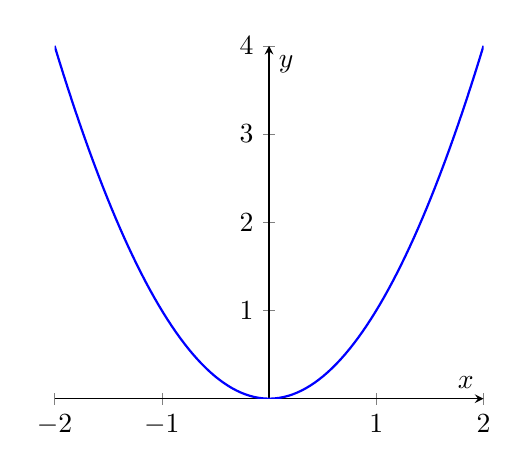
\begin{tikzpicture}
    \begin{axis}[
        axis lines = middle,
        xlabel = $x$,
        ylabel = {$y$},
        samples = 100,
        domain = -2:2,
        ymin = 0, ymax = 4,
        xmin = -2, xmax = 2,
        width = 200
    ]
    \addplot[blue, thick] {x^2};
    \end{axis}
    \end{tikzpicture}
    \caption{Plot of $y = x^2$.}
    \end{figure}
On the contrary, $f(x) = x$ is a one to one and onto function. We call a function like this \textbf{Bijective}



\begin{figure}[!h]
    \centering
    \begin{tikzpicture}
    \begin{axis}[
        axis lines = middle,
        xlabel = $x$,
        ylabel = {$y$},
        samples = 100,
        domain = -2:2,
        ymin = -2, ymax = 2,
        xmin = -2, xmax = 2,
        width = 200
    ]
    \addplot[blue, thick] {x};
    \end{axis}
    \end{tikzpicture}
    \caption{Plot of $y = x^2$.}
    \end{figure}


\subsubsection{Hash Function}
A hash function is defined from a larger, possibly infinite, set of data to a smaller fixed-size set of integers. For example, let $h:\Z^+ \to \{0,1\}$ such that, for any $k \in \Z^+$
\[
h(k) = \begin{cases}
    0 \quad k \notin 2\Z \\
    1 \quad k \in 2\Z
\end{cases}
\]
For example, the Dirichlet function is defined as $f: \R \to \{0,1\}$ such that, for any $x \in \R$,
\[
f(x) = \begin{cases}
    0 \quad x \in \R - \Q \\
    1 \quad x \in \Q
\end{cases}
\]



\subsubsection{Theorem 7.2.2}
Suppose $f\colon X \to Y$ is a bijection. Then there is a function $f^{-1} \colon Y \to X$ such that
\[
f^{-1}(y) = x \iff y = f(x)
\]
$f^{-1}$ is called the inverse function of the function $f$


\subsubsection{Properties of Exponents}
\begin{align*}
    b^xb^y = b^{x+y}\\
    \paren{b^x}^y = b^{xy}\\
    \paren{ab}^x = a^xb^x
\end{align*}
\subsubsection{Logarithmic and Exponential Function}
We can use the unique factorization for the integers and the definition of logarithm to prove that something like $\log_37$ is irrational.
            \begin{proof}
                let $x \in \R : x = \log_3 7$ by definition of logarithm, we can rewrite $x=\log_3 7$ as 
                    \[
                    3^x = 7
                    \]
                by the unique factorization theorem, every integer greater than 1 is either a prime or equals to a unique combination of prime. Suppose $x$ is rational, then $x = \frac{m}{n}$ for some $m \in \Z$ and $n \in \Z - \zero$. We can rewrite the expression as
                    \[
                    3^\frac{m}{n} = 7
                    \]
                raising both side to the power of $n$, we have
                    \[
                    3^n = 7^n
                    \]
                Since this equation has no integer solution except for $n=0$, which is not within the allowed range for $n$. Therefore this is a contradiction from the assumption that $x$ is rational. We can therefore conclude that $x$ is irrational. 
            \end{proof}   



\subsection{Composition of Functions}
Let $f \colon X \to Y_1$ and $g \colon Y_2 \to Z$ such that $f(X) \subseteq Y_2$. Define $g \circ f \colon X \to Z$ such that for any $x \in X$, 
\[
\paren{g \circ f}(x) = g\paren{f(x)}
\]
the function $g \circ f$ is called \textbf{the composition of $f$ and $g$}

\subsubsection{Theorem 7.3.3}
If $f \colon X \to Y$ and $g \colon X \to Y$ are both injective functions, then $g \circ f$ is injective. 
\begin{proof}
    let $f \colon X \to Y$ and $g \colon X \to Y$ be injective functions. Suppose $ f(x_1) = f(x_2)$, $g(f_1) = g(f_2)$. Then $f(x_1)=f(x_2)$ since $g$ is injective. since $f$ is injective, then $g(f_1) = g(f_2)$, therefore $g \circ f$ is injective. 
\end{proof}

\subsubsection{Theorem 7.3.19}
If $f \colon X \to Y$ and $g \colon X \to Y$ be any functions, suppose $g \circ f$ is injective. Is $g$ or $f$ injective.
\begin{proof}
 let $f \colon X \to Y$ and $g \colon X \to Y$ be injective functions. Suppose $g \circ f(x_1) = g \circ f(x_2)$. Suppose $f(x_1) = f(x_2)$, since 
    
\end{proof}


\subsubsection{Theorem 7.3.4}
If $f \colon X \to Y$ and $g \colon X \to Y$ are both surjective functions, then $g \circ f$ is surjective.

\begin{proof}
    let $f \colon X \to Y$ and $g \colon X \to Y$ be any surjective functions. let $z \in \Z$ since $g$ is surjective, there exists $y \in Y$
\end{proof}


\subsubsection{A Set-theoretic Notation}
Let $Y^X$ denote the set of all functions from a domain set $X$ to a codomain set $Y$.
\[
N\paren{Y^X} = N\paren{Y}^{N\paren{x}} = \abso{Y^X} = \abso{Y}^{\abso{X}}
\]

\subsubsection{Pigeonhole Theorem} 
Let $X,Y$ be sets such that $N(X) = n \in Z^+$ and $N(Y) = m \in \Z^+$. For any $f \in Y^X$, if $n >m$ then $f$ is not injective. 

\subsubsection{Generalized Pigeonhole Theorem}
For any function $f$ from a finite set $X$ with $n$ elements to a finite set $Y$ with $m$ elements and , for any positive integer $k$, if $km <n$, then there is some $y\in Y$ such that y is the image of at least $k+1$ distinct elements of $X$.

Let $X,Y$ be sets such that $N(X) = n \in \Z^+$, and $N(Y) = m \in \Z^+$, for any $f \in Y^X$, and $k \in Z^+$, if $n >km$ then there exists $y \in Y$ such that $N\paren{f^{-1}(y)} \geq k+1$, where $f^{-1}(y) = \{ x\in X \colon f(x) = y\}$

The Generalized Pigeonhole Theorem essentially states that if you try to map a larger set into a smaller set, there must be at least one element in the smaller set that is the image of multiple elements from the larger set. Let's go through an example to make this clearer.

\textbf{Example:}

Let \( X = \{1, 2, 3, 4, 5, 6, 7\} \) be a set with \( n = 7 \) elements, and let \( Y = \{a, b, c\} \) be a set with \( m = 3 \) elements. Consider the function \( f: X \rightarrow Y \).

Let \( k = 2 \), so \( km = 2 \times 3 = 6 \). Since \( n = 7 \) and \( 7 > 6 \), according to the Generalized Pigeonhole Theorem, there must be some element \( y \in Y \) such that \( f^{-1}(y) \) contains at least \( k + 1 = 3 \) elements.

\textbf{Function Example:}

Let's define the function \( f \) as follows:
\[
f(1) = a, \quad f(2) = a, \quad f(3) = a, \quad f(4) = b, \quad f(5) = b, \quad f(6) = c, \quad f(7) = c
\]

In this case:
\begin{align*}
f^{-1}(a) &= \{1, 2, 3\}, \quad \text{so} \quad N(f^{-1}(a)) = 3 \\
f^{-1}(b) &= \{4, 5\}, \quad \text{so} \quad N(f^{-1}(b)) = 2 \\
f^{-1}(c) &= \{6, 7\}, \quad \text{so} \quad N(f^{-1}(c)) = 2
\end{align*}

Here, \( f^{-1}(a) \) contains 3 elements, which is at least \( k + 1 = 3 \), satisfying the theorem. Therefore, the function \( f \) demonstrates the Generalized Pigeonhole Theorem, as there exists at least one element in \( Y \) (in this case, \( a \)) that is the image of at least \( k + 1 = 3 \) distinct elements from \( X \).
\subsubsection{Definition 8.3.1}
A \textit{Partition} $S$ of a set $X$ is a set of nonempty and mutually disjoint subsets of $X$ such that $X$ is a disjoint union of the subsets.
\begin{enumerate}
    \item $\varnothing \notin S$
    \item $\bigcup_{X_i \in S}^{}X_i = X$
    \item For all $X_i,X_j \in S$, $X_i \neq X_j \implies X_i \cap X_j = \varnothing$
\end{enumerate}

\subsection{Relation}


\subsubsection{Equivalence Relation}
Let $A$ be a set and $R$ a relation on $A$. $R$ is an \textbf{equivalence relation} if and only if $R$ is reflexive, symmetric, and transitive. 

\subsubsection{Equivalence Class}
Suppose $A$ is a set and $\sim$ is an equivalence relation on $A$. For all $a \in A$, the equivalence class of $a$, denoted $[a]$, and called the class of $a$ for short, is the set of all elements $x \in A$ such that $x \sim a$, i.e. $[a] = \{ x\in A \colon x \sim a\}$

\subsubsection{Lemma 8.3.2}
Suppose $A$ is a set, $\sim$ is an equivalence relation on $A$, and $x,y$ are elements of $A$. If $x \sim y$ then $[x] = [y]$
\begin{proof}
    Suppose $A$ is a set, and $\sim$ is an equivalence relation on $A$, and $x,y$ are elements of $A$. Suppose $x \sim y$. Suppose $a\in[x]$, then $a \in [y]$ since $x \sim y$ is transitive. therefore $[x] \subseteq [y]$. 
    Since $x \sim y$, then $y \sim x$ via symmetry. Then suppose $b \in [y]$, then $b\in [x]$ via transitivity. Therefore $[y] \subseteq [x]$. therefore 
    \[
    [x]=[y]
    \]
\end{proof}

\subsubsection{Lemma 8.3.3}
If $A$ is a set, $\sim$ is an equivalence relation on $A$ and $x,y$ are elements of $A$, then 
\[
[x] \cap [y] = \varnothing \vee [x] = [y]
\]
\begin{proof}
    Suppose $A$ is a set, and $\sim$ is an equivalence relation on $A$, and $x,y$ are elements of $A$. We can say
    \[
    [x]\cap [y] = \varnothing \quad \vee \quad [x]\cap [y] \neq \varnothing
    \]
    Suppose $[x]\cap [y] = \varnothing$. Then $[x]\cap [y] = \varnothing$ or $[x]=[y]$ via generalization. Now suppose $[x]\cap [y] \neq \varnothing$. Then there exists $u \in [x]\cap [y]$. And $u \in [x]$ and $u \in [y]$. Therefore $u \sim x$ and $u \sim y$. Since $\sim$ is symmetric, $x\sim u$. $x\sim u$ and $u \sim y$ therefore $x \sim y$ by transitivity. By lemma 8.3.2, so $[x] = [y]$. And $[x] = [y]$ or $[x] \cap [y] = \varnothing$ by generalization. 
\end{proof}

\subsubsection{Lemma 8.3.4}
If $A$ is a set and $\sim$ is an equivalence relation on $A$, then the distinct equivalence classes of $\sim$ form a partition of $A$; meaning the union of the equivalence classes is all of $A$, and the intersection of any two distinct classes is empty. 
\begin{proof}
    Let $A$ be a nonempty set, and $\sim$ an equivalence relation on $A$. Let $n \in \Z^+$ and $\{A_1, A_2, \ldots , A_n\}$ be the set of distinct equivalence classes of $A$. We need
    \[
    A = \bigcup_{i=1}^{n}A_i = \{ x \in U \colon \exists i \in \{1,\ldots,n\} \paren{x \in A_i}\}
    \]
    We need to show
    \[
    A \subseteq \bigcup_{i=1}^{n}A_i  \quad \wedge \bigcup_{i=1}^{n}A_i  \subseteq A
    \]
    We also need
    \[
    \forall i,j \in \{1,\ldots n\}\paren{i \neq j \then A_i \cap A_j = \varnothing}
    \]
    We let $a \in \bigcup_{i=1}^{n}A_i$, then there exists $j \in \{1,\ldots n\} $ such that $a \in A_j$ Since $A_j$ is an equivalence class of $A$, then $a \in A_j \then a \in A$. Therefore
    \[
    \bigcup_{i=1}^{n}A_i  \subseteq A
    \]
    Now, let $a \in A$, since $\sim$ is an equivalence relation, $a \sim a$. Then $a \in [a] = \{ x \in A \colon x\sim a\}$. Since $\{A_1,A_2, \ldots,A_n\}$ is the set of all distinct equivalence classes of $A$, then
    \[
    a \in [a] \cap A_j \supseteq \{a\} \neq \varnothing
    \]
    for some $j \in \{1,\ldots,n\}$. Since $[a] \cap A_j$ via lemma $8.3.3$. So there is some $j$ such that $a \in A_j$ and $a \in \bigcup_{i=1}^{n}A_i  $, and since $a \in A$, then 
    \[
    A \subseteq  \bigcup_{i=1}^{n}A_i .
    \]
    This concludes
    \[
    A = \bigcup_{i=1}^{n}A_i 
    \]
    Now we let $i,j \in \{1,\ldots,n\}$. Suppose $i \neq j$. We want to show $A_i \cap A_j = \varnothing$. Suppose $A_i \cap A_j \neq \varnothing$, then by lemma 8.3.3, $A_i = A_j$ via elimination, this contradicts with the claim that they are distinct classes, therefore $A_i \cap A_j = \varnothing$ by contradiction. 
\end{proof}


\subsubsection{Congruence Modulo}
Let $n \in \Z^+$. Let $\sim$ be the relation of congruence modulo $n$ on $\Z$, i.e. for any $k,l \in \Z$
\[
k \sim l \iff n \mid (k-l)
\]
We can see the equivalence classes of $\sim$ for any $k \in \{0,1,2,\ldots, n-1\}$, is basically all the remainders possible from the modulus operation with $n$.

\subsubsection{Congruent}
Let $k,l \in \Z$, and let $n \in \Z^+$. $l$ is congruent to $k$ modulo $n$, written 
\[
l \equiv k (\bmod \; n),
\]
if and only if $n \mid (l-k)$.
\[
l \equiv k (\bmod \; n) \iff n \mid (l-k)
\]

\subsubsection{Example 8.3.finale}

define $\sim$ to be a relationship as follow
\[
(a,b) \sim (c,d) \iff ad=bc
\]

\begin{proof}
    We need to prove $\sim$ is reflexive
    \[
    \forall q \in A (q \sim q)
    \]
    Symmetric
    \[
    \forall p,q \in A( p \sim q \then q \sim p)
    \]
    And transitive
    \[
    \forall p,q,r \in A ( p\sim q \wedge q\sim r \then p \sim r)
    \]
    We prove the reflexivity first. Let $q \in A$, which means $q = (a_1,b_1)\in \Z \times \paren{\Z - \zero}$. We have
    \[
    (a_1,b_1) \sim (a_1,b_1)
    \]
    we see that $a_1b_1 = a_1b_1$, and that is true. Now we need to prove it being transitive. We ,et $p,q \in A$. let $p = (a_1,b_1)\in \Z \times \paren{\Z - \zero}$ and $q = (a_2,b_2)\in \Z \times \paren{\Z - \zero}$. Suppose $p \sim q$, then 
    \[
    a_1b_2 = b_1a_2
    \]
    from this, we can obtain $a_2b_1 = b_2a_1$, which means $q \sim p$. So $\sim $ is symmetric. Now we need to prove its transitive. We let $p,q,r \in A$, we have
    \begin{align*}
        p = (a_1,b_1)\in \Z \times \paren{\Z - \zero}\\
        q = (a_2,b_2)\in \Z \times \paren{\Z - \zero}\\
        r = (a_3,b_3)\in \Z \times \paren{\Z - \zero}
    \end{align*}
    Suppose $p \sim q$ and $q \sim r$. Since $p \sim q$, then $a_1b_2 = b_1a_2$. And since $q \sim r$, we have $a_2b_3 = b_2a_3$. If we work on the equality, we obtain
    \[
    a_1b_2b_3 = b_1a_2b_3
    \]
    by multiplying $b_3$ on both side of $p \sim q$, and 
    \[
    b_1a_2b_3 = b_1b_2a_3
    \]
    by multiplying $b_1$ on both side of $q \sim r$. Since equality on $\Z$ is transitive, then 
    \[
    a_1b_2b_3 = b_1a_2b_3 = b_1b_2a_3
    \]
    Now we divide both side by $b_2$ since $b_2$ is not zero, then we have $a_1b_3 = b_1a_3$, which means $p \sim r$. Therefore if $p \sim q$ and $q \sim r$, then $p \sim r$ or $\sim$ is transitive. 


    
    

    
\end{proof}




\end{document}


